%%%%%%%%%%%%%%%%%%%%%%%%%%%%%%%%%%%%%%%%%%%%%%%%%%%%%%%%%%%%%%%%%%%%%%%%%%%%%%%%%%%%%%%%%%%%%%%%%%%%%
% This template is distributed with ABSOLUTELY NO WARRANTY.
% It serves as a guideline and constitutes a basic structure for a
% thesis/dissertation. The user assumes full responsibility for formatting
% and typesetting their document and for verifying that all the thesis
% requirements set by the University of Tennessee are met. Please refer to the most
% recent UT thesis guide (http://gradschool.utk.edu/thesesdissertations/formatting/)
% or contact the thesis consultant (http://gradschool.utk.edu/thesesdissertations/).
% Please report any bugs to the thesis consultant.
%%%%%%%%%%%%%%%%%%%%%%%%%%%%%%%%%%%%%%%%%%%%%%%%%%%%%%%%%%%%%%%%%%%%%%%%%%%%%%%%%%%%%%%%%%%%%%%%%%%%%
% O P T I O N S:
% 1. thesis/dissertation
% 2. monochrome
% 3. all options provided by the report class
%%%%%%%%%%%%%%%%%%%%%%%%%%%%%%%%%%%%%%%%%%%%%%%%%%%%%%%%%%%%%%%%%%%%%%%%%%%%%%%%%%%%%%%%%%%%%%%%%%%%%
%First, is this a thesis or dissertation? Choose one by commenting out the one you don't need:
%\documentclass[thesis,letterpaper,12pt]{utthesis} % thesis
\documentclass[dissertation,letterpaper,12pt]{utthesis} %dissertation
% some alternatives are:
%\documentclass[thesis,monochrome,letterpaper,12pt]{utthesis} %thesis, monochrome text
\renewcommand{\baselinestretch}{1.5} 	 % line Spacing
%%%%%%%%%%%%%%%%%%%%%%%%%%%%%%%%%%%%%%%%%%%%%%%%%%%%%%%%%%%%%%%%%%%%%%%%%%%%%%%%%%%%%%%%%%%%%%%%%%%%%
% TO DO: FILL IN YOUR INFORMATION BELOW - READ THIS SECTION CAREFULLY
%%%%%%%%%%%%%%%%%%%%%%%%%%%%%%%%%%%%%%%%%%%%%%%%%%%%%%%%%%%%%%%%%%%%%%%%%%%%%%%%%%%%%%%%%%%%%%%%%%%%%
\title{On the Resilience of Supply Chain Design under Disruptions}	       	% title of thesis/dissertation
\author{Samarth Shashank Vagal}                			% author's name
\copyrightYear{2019}            				% copyright year of your thesis/dissertation
\graduationMonth{May}           				% month of graduation for your thesis/dissertation
\degree{Master of Science}	    			% degree: Doctor of Philosophy, Master of Science, Master of Engineering...
\university{The University  of Tennessee, Knoxville}	% school name
%%%%%%%%%%%%%%%%%%%%%%%%%%%%%%%%%%%%%%%%%%%%%%%%%%%%%%%%%%%%%%%%%%%%%%%%%%%%%%%%%%%%%%%%%%%%%%%%%%%%%
% LOAD SOME USEFUL PACKAGES. 
% No need to change anything here, although if you'd like to add packages you can do that here. Note that packages preloaded with the utthesis class are: amsmath,amsthm,amssymb,setspace,geometry,hyperref,and color
%%%%%%%%%%%%%%%%%%%%%%%%%%%%%%%%%%%%%%%%%%%%%%%%%%%%%%%%%%%%%%%%%%%%%%%%%%%%%%%%%%%%%%%%%%%%%%%%%%%%%
\usepackage{nomencl}                    % produces a nomenclature
\usepackage{float}                      % figure floats
\usepackage[numbers]{natbib}                     % this package allows you to link your references
\usepackage{graphicx}					% graphics package
\graphicspath{ {figures/}{figures/eps/}{figures/pdf/} }% specify the path where figures are located
\usepackage{fancyhdr}                   % fancy headers and footers
\usepackage{url}                        % nicely format url breaks
\usepackage[inactive]{srcltx}		 	% necessary to use forward and inverse searching in DVI
\usepackage{relsize}                    % font sizing hierarchy
\usepackage{booktabs}                   % professional looking tables
\usepackage[config, labelfont={bf}]{caption,subfig} % nice sub figures
\usepackage{mathrsfs}                   % additional math scripts
\usepackage[titletoc]{appendix}			% format appendix correctly
\usepackage{pdflscape}					% to produce landscape pages if necessary

%%%%%%%%%%%%%%%%%%%%%%%%%%%%%%%%%%%%%%%%%%%%%%%%%%%%%%%%%%%%%%%%%%%%%%%%%%%%%%%%%%%%%%%%%%%%%%%%%%%%%%
% This section formats landscape pages properly with the correct page number.
% This code is only necessary when landscape pages are needed and can be left alone
%%%%%%%%%%%%%%%%%%%%%%%%%%%%%%%%%%%%%%%%%%%%%%%%%%%%%%%%%%%%%%%%%%%%%%%%%%%%%%%%%%%%%%%%%%%%%%%%%%%%%%

\fancypagestyle{mylandscape}{
	\fancyhf{} %Clears the header/footer
	\fancyfoot{% Footer
    \makebox[\textwidth][r]{% Right
      \rlap{\hspace{.75cm}% Push out of margin by \footskip
        \smash{% Remove vertical height
          \raisebox{4.87in}{% Raise vertically
            \rotatebox{90}{\thepage}}}}}}% Rotate counter-clockwise
  \renewcommand{\headrulewidth}{0pt}% No header rule
  \renewcommand{\footrulewidth}{0pt}% No footer rule
}


%%%%%%%%%%%%%%%%%%%%%%%%%%%%%%%%%%%%%%%%%%%%%%%%%%%%%%%%%%%%%%%%%%%%%%%%%%%%%%%%%%%%%%%%%%%%%%%%%%%%%
\begin{document}
    \pagenumbering{alph} % this is needed to clear certain issues with the hyperref package
    %
    \addToPDFBookmarks{0}{Front Matter}{rootNode} % create a root node named "Front Matter" in the pdf bookmarks
    \addToPDFBookmarks{1}{Title}{a} % add a pdf bookmark to the title page
    \makeTitlePage % make the title page.
    %
    \pagenumbering{roman}
    \setcounter{page}{2}
    %
    \makeCopyrightPage % make the copyright page
    %
%%%%%%%%%%%%%%%%%%%%%%%%%%%%%%%%%%%%%%%%%%%%%%%%%%%%%%%%%%%%%%%%%%%%%%%%%%%%%%%%%%%%%%%%%%%%%%%%%%%%%
%The dedication and acknowledgments are optional. If you wish not to include them, simply comment out both the "\addToPDF..." line and the "\include{...}" line for each.
%%%%%%%%%%%%%%%%%%%%%%%%%%%%%%%%%%%%%%%%%%%%%%%%%%%%%%%%%%%%%%%%%%%%%%%%%%%%%%%%%%%%%%%%%%%%%%%%%%%%%
    \addToPDFBookmarks{1}{Dedication}{b} % add a pdf bookmark to the dedication page
    \chapter*{}
\begin{center}
{\centering \it I would like to dedicate this thesis to my loving family who have been my backbone all throughout my life. Their emotional and moral support guided me at every step in life. Even being miles away, a conversation with them every night gave me the strength to get through the tough times.}
\end{center}  % include the dedication

    \addToPDFBookmarks{1}{Acknowledgments}{c} % add a pdf bookmark to the acknowledgments page
    \chapter*{Acknowledgments}
I would like to thank the following people for playing a significant role towards the completion of this thesis:

\textbf{My Committee:} My advisor Dr. Li helped me through each and every step of the thesis. He mentored me in developing the approach to solve the problem at hand. He made sure that my doubts would get solved at any time of the day. Thanks to his support, and the support of Dr. Kobza and Dr. Lee Martin, I was able to complete the thesis and my Master's degree. 

\textbf{My Parents:} I would again like to thank my parents because without them nothing would have been possible. 

\textbf{The University of Tennessee:}I am grateful to the UTK to take me in as one of their student and help me pursue my dreams.

\textbf{My friends:} I would like to acknowledge my friends for helping me get through the difficult times spent away from home. They made me feel like this was my home away from home. % include the acknowledgments
    
    \addToPDFBookmarks{1}{Abstract}{e} % add a pdf bookmark to the abstract page
    \chapter*{Abstract}\label{ch:abstract}
 It is not possible to design a system in which there are no failures. To make the system more efficient, it is important to design the system in such a way that once the failure has occurred, the system can be restored to its full functionality in a short span of time. For a system to perform this task, we need to make the system "resilient". The basic idea of resilience is the ability to recover from an occurred failure in a system so that the system is performing at its best level. Resilience can be applied to all types of systems. This study aims at enhancing the resiliency of Supply Chains in the event of disruption at various levels. Supply Chains are one of the most important aspects for the growth and welfare of any business. Supply chain, just like any other system, is prone to disruption. A supply chain disruption is an unanticipated event that slows down the normal flow or even stops the normal flow of materials with hampering effects to the members within the supply chain. For enhancing the resiliency, various tools such as contingency planning, key indicators identification, and simulation have been implemented through the aggregate dimensions. The simulation tool is incredibly helpful for designing different scenarios in the highly complex supply chains. This study also sheds light on how the disruptions are transmitted through the various members of the supply chain and through different levels. The contingency planning plays an important role in the time of disruption by providing alternate sourcing ideology so that the supply chain does not come at a halt and costs the firm losses in terms of money and time. % your abstract  
     
    \addToPDFBookmarks{0}{Table of Contents}{f}
    \tableofcontents % generate a table of contents
    \listoftables % generate a list of tables
    \listoffigures % generate a list of figures
   
    \newpage
    \pagenumbering{arabic}
    \setcounter{page}{1}
    %%%%%%%%%%%%%%%%%%%%%%%%%%%%%%%%%%%%%%%%%%%%%%%%%%%%%%%%%%%%%%%%%%%%%%%%%%%%%%%%%%%%%%%%%%%%%%%%%%%%%
    % INCLUDE THE CHAPTERS STARTING WITH THE NOMENCLATURE IF PRESENT
    %%%%%%%%%%%%%%%%%%%%%%%%%%%%%%%%%%%%%%%%%%%%%%%%%%%%%%%%%%%%%%%%%%%%%%%%%%%%%%%%%%%%%%%%%%%%%%%%%%%%%
    \include{front-matter}
    \chapter{Introduction} \label{ch:introduction}
 In a world full of constant uncertainties and disruptions, it is quintessential to have a sense of awareness and preparedness in order to avoid the losses or keep the losses as minimum as possible. The ability of a firm to withstand such uncertainties/disruptions and maintain the operational performance proves to have an advantage over the competitors. To comprehend the impact of these disruptions in the supply chains of firms, we need to have a fundamental understanding of several concepts first. These concepts include resilience, robustness, SC resilience and robustness, disruption propagation, network structure of the supply chain, and the implementation of simulation in supply chain design. The elaboration on these concepts is made in this chapter in the following sections.

\section{The Concept of Resilience and Robustness}
The fundamental idea of resilience has a foundation in almost all fields. In the article published by (\citeauthor{Boin2010}, \citeyear{Boin2010}) resilience can be observed in the fields such as engineering, biology, and psychiatry. Even though they have different meanings in their particular domains, the idea of resilience remains the same. Another definition as put by (\citeauthor{Westrum2006}, \citeyear{Westrum2006}) states that resilience is the ability prevent something bad from happening, ... to prevent something bad from becoming worse, or ... the ability to recover from something bad once it has happened.  (\citeauthor{HaleA.&Heijer2006}, \citeyear{HaleA.&Heijer2006}) define resilience as, ``...the ability in difficult conditions to stay within the safe envelope and avoid accidents". 

The resilience triangle is shown in Fig \ref{Resilience Triangle}. The quality of infrastructure percentage can be replaced by system performance to keep it as a generic measure. The main target over here is to keep the triangle as small as possible i.e the length between time $t_{\text{0}}$ and $t_{\text{1}}$ should be made as minimum as possible for a system to be highly resilient. There are many strategies that can be implemented to shorten the time length. The strategy that has been used in our study is a mix of contingency planning and key indicators identification. The implementation of these strategies is exhibited in the latter sections of our study.


Robustness has been defined by (\citeauthor{Tierney2007}, \citeyear{Tierney2007}) as ``the ability of systems, system elements,
and other units of analysis to withstand disaster
forces without significant degradation or loss of
performance". In simpler words, if the system is robust, then it should be able to continue its operations in the face of disruptions. The system does not exhibit robustness on its own. There are certain modifications that need to be occurred at the time of disruption at various levels by using methods of forecasting and planning. If these decisions are not taken at the intended time, then the system fails to obtain the state of robustness. 

\begin{figure}
  \centering
  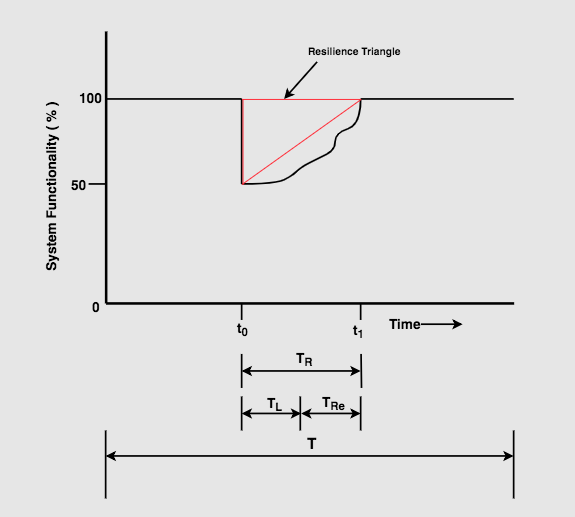
\includegraphics[width=6.5in]{figures/pdf/Resilience-Triangle.png}\\
  \caption{Resilience Triangle} \label{Resilience Triangle}
\end{figure}

\newpage
\section{Resilience and Robustness in Supply Chain}
Now that the understanding of the concepts of resilience and robustness has been established, let us incorporate these concepts into supply chain and find the significance they hold. The primary definitions for these concepts remain the same, but the supply chain is considered as our system in this case. (\citeauthor{Brandon-JonesE.;SquireB.;Autry2014},  \citeyear{Brandon-JonesE.;SquireB.;Autry2014})  have defined SC Resiliency as `` the ability of a system to return to its original state, within an acceptable period of time, after being disrupted". Resilience aids in indicating the weakest links of the chain and fortify them such that in the event of a similar disruption in the future, the system would be easily able to deal with it. (\citeauthor{Kitano2004}, \citeyear{Kitano2004}) defines SC Robustness as ``the ability of the supply chain to maintain its function despite internal or external disruptions".

These two concepts are coming into the light and  starting to have a pivotal role in the enhancement in the performance of the system due to rise in the number of uncertainties and unanticipated natural disasters. Incorporating these two factors into a supply chain would give the competitive advantage over others in the highly complex market.

SC resiliency and robustness ensures that there is a constant flow of materials and information throughout the supply chain. Even a hold up of materials in any facility within a SC of the firm makes a huge impact in terms of both time and money. Along with this, there are chances that the customer may decide to change to other firms due to the dissatisfaction caused to them. Various big companies such as Proctor and Gamble, Coca-Cola, Boeing, and Cisco have shifted their attention towards the implementation of resilience and robustness in their supply chains. 

\newpage
\section{Disruption Propagation}
Considerable research has been invested in understanding, predicting, preventing, and managing disruptions  (\citeauthor{Ivanov2016}, \citeyear{Ivanov2016}). The propagation of the disruption within a supply chain directly impacts the outcome. It is of utmost importance to focus on the supply chain disruption propagation because as the disruption spreads, the negative effects disseminate throughout the supply chain until the whole system fails. It is necessary to address the disruption at any level irrespective of its magnitude. A disruption which may seem innocuous has the potential to turn into a critical and harmful disruption by propagating and amplifying through various levels of the supply chain. The factors that affect the propagation of the supply chain disruption should be comprehended for better addressing of the disruptions.

The qualitative analysis made through the Gioia methodology mentioned by (\citeauthor{Scheibe2017}, \citeyear{Scheibe2017}) validates the data analysis to be done in three different orders. The first order analysis describes and summarizes the data. The second order analysis reduces the data by grouping similar codes and descriptions. The third order analysis consolidates the second-order themes into logical groupings called aggregate dimensions. There are three aggregate dimensions having two second-order themes each. These aggregate dimensions are 

1) Nature of the Disruption

2) Supply Chain Structure and Dependence 

3) Managerial Decision Making

The nature of the disruption itself affects the severity of the propagation of the disruption. The better understanding of the nature of the disruption poses as the foundation element in managing the disruption propagation. The two second-order themes associated with the nature of the disruption are correlation of risks and compounding effects. The correlation of risks theme states that one risk or even a risk mitigation strategy can inflict another risk. The disruptions never happen in a single member along a supply chain. Due to the strong interdependent and connected nature of the supply chain, disruptions never occur as an isolated event. The compounding effect means the adhering of one disruption to other as it propagates along the supply chain. Due to the compounding effect, the disruptions grow in size and severity. The decision-making capability of the stakeholders directly contributes to the compounding effect. Self-preservation or measures to mitigate the risk at a personal level increases the severity of the disruption. The structure of the supply chain and the consisting dependencies serve as a source of propagation of disruption along the supply chain.

The two second-ordered themes associated with the supply chain structure and dependence are cyclical linkages and counterparty risk as shown in Fig \ref{Aggregate Dimensions}. The cyclical linkages are nothing but the inter-dependencies between the nodes of a supply chain. A problem in one node leads to a problem in another node and vice versa. These linkages often go unnoticed until the disruptions occur. The cyclical linkages occur as a reason of one or more members playing different roles at different levels in the same supply chain. To mitigate the supply chain disruption propagation, the cyclical linkages must be carefully observed and studied. Counterparty risk occurs when one supplier supplies to a firm and its competitor at the same time. This means that the risk in one link in the supply chain is dependent on the other link. It is arduous to identify the interconnection through which the disruption can propagate. The firm focuses on one interconnection within a supply chain when the risk through different parts of the supply chain hit the firm without having any knowledge of it. The counterparty risk takes place mainly due to the hiding of information within the supply chain members (\citeauthor{Scheibe2017}, \citeyear{Scheibe2017}). 

The managerial decision-making at the time of disruptions also affect the propagation through the supply chain. The two-second ordered themes associated with this type of aggregate dimension are herding behavior and misaligned incentives as shown in Fig \ref{Aggregate Dimensions} (\citeauthor{Scheibe2017}, \citeyear{Scheibe2017}). The herding behavior is the behavior in which one person behaves the way that others behave even though they are completely different people. In case of a supply chain, during the time of disruption, a firm takes the same measures as others are taking to mitigate the disruption although they have different properties and structure. They just tend to follow the 'herd' without thinking. The easiest example of herding behavior is when food joints adjust their prices based on other food joints which are the competitors. Misaligned incentives are the decisions made by the supply chain decision-makers which benefits one part of the supply chain at the expense of the other parts in the supply chain. These decisions are a result of the inability of the decision-makers to see the bigger picture and improve the entire supply chain rather than improving just one part of it. One such misaligned incentive is giving more importance to taking actions after a disruption takes place rather than taking actions to avoid the disruption from happening. 


\begin{figure}[H]
  \centering
  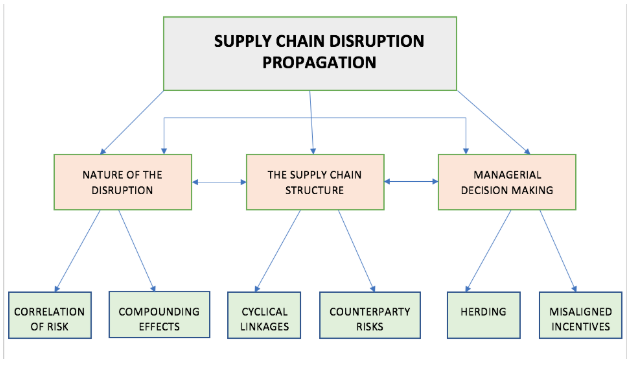
\includegraphics[width=4.5in]{figures/pdf/Aggregate-Dimensions.png}\\
  \caption{Aggregate Dimensions and their Second-order themes.}\label{Aggregate Dimensions}
\end{figure}

In a supply chain, the aggregate dimensions are the major source of the disruption propagation. If the risks in these aggregate dimensions are mitigated and the supply chain is designed in such a way that it would avoid any disruption propagation, then the resiliency of the supply chain is increased. There has been ample research related to the identification of the risks associated with the aggregate dimensions but there has not been a lot of research in the field of mitigation of the disruption propagation through the aggregate dimensions (\citeauthor{Scheibe2017}, \citeyear{Scheibe2017}). The nature of disruption, supply chain structure, and managerial decisions are the aggregate dimensions through which the supply chain disruption propagation can be contained.

The Figure \ref{Aggregate Dimensions} represents the aggregate dimensions on which the supply chain disruption propagation is dependent on. It also shows the second order themes which contribute to the aggregate dimensions. Out of these, correlation of risk and cyclical linkages have a significant impact on the disruption propagation. Hence, the main focus of this paper would be to model a supply chain in such a manner that the problems arising in the supply chain due to these factors could be anticipated and mitigated at the initial stages to avoid cascading of the failure through the supply chain.

\subsection{Correlation of Risks}
The supply chain is a network of strongly interconnected nodes which function together in coordination for getting the desired output. If there is a disruption occurring at any level in the supply chain, it is plausible to affect the performance of the supply chain. It is observed that this disruption does not just affect the point of occurrence, but it may be propagated throughout the SC because of the inter-connectivity. The disruption may travel upstream as well as downstream the SC. This phenomenon is called as the ripple effect in the supply chain (\citeauthor{ivanov2017simulation}, \citeyear{ivanov2017simulation}). It is highly unlikely for a disruption to occur in isolation. It is not just the risk that can cause another risk, but the strategy to mitigate one risk can also lead to risk in a different node in the SC. Thus, the risk mitigation strategy should not be focused only on reducing the risk at a certain point, but it should also pay close attention towards the effects of the risk as well as the effects of the mitigation technique on other elements of the SC.

The Figure \ref{Ripple effect} represents the ripple effect in a supply chain structure. It can be evidently seen that the disruption is going to propagate in both directions. It is important to minimize the risk caused due to the disruption. At the same time, the risks associated with the mitigation strategy should also be taken into consideration. The decisions that are taken once the disruption occurs play a vital role in the degree of recovery of the SC. The managerial decisions during disruption about these decision variables and the ripple effect analysis throughout the SC will contribute towards the resilience of the SC.

The methodology that has been suggested for limiting the propagation of risks due to the correlation of risks is the ripple effect modeling. With the help of this methodology, the effect of the disruption and the effect of the strategies devised to reduce the risks due to the disruption can be found out throughout the supply chain structure. This will help in making the supply chain more resilient by reducing the risks after the disruption has occurred.

\begin{figure}[H]
  \centering
  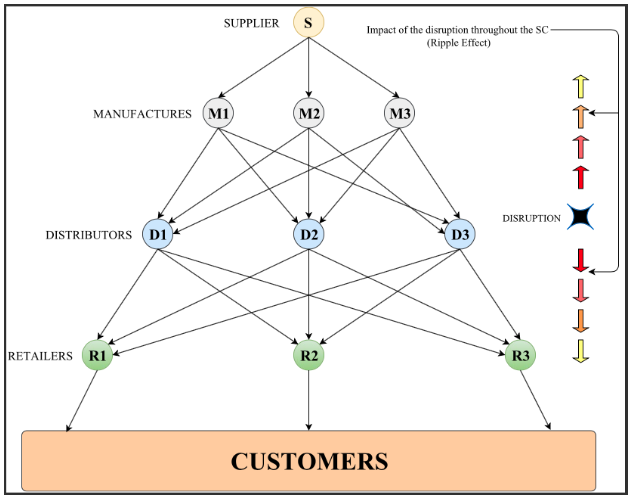
\includegraphics[width=6.5in]{figures/pdf/Ripple-effect.png}\\
  \caption{Ripple effect in the Supply Chain Structure.}\label{Ripple effect}
\end{figure}

\newpage
\subsection{Cyclical Linkages}

In a supply chain, all the nodes are inter-connected and are inter-dependent. This aids in the desired functioning of the supply chain. At the same time, if there is any disruption in the SC, the same inter-connectivity and inter-dependence will become disadvantageous. Suppose that there are three nodes in a supply chain. If there is a problem in node 1, then it can transmit a problem to node 2. Similarly, if there is a problem in node 2, it may propagate to node 3. The problem in node 3 can have a feedback effect on the first node. This is called as the cyclical linkage in supply chain and is shown in Fig \ref{Cyclical Linkage}. A disruption in one of the stages of trade-off can lead to a disruption in the other stages due to the cyclical linkage. Thus affecting the entire supply chain at different levels.

\begin{figure}[H]
  \centering
  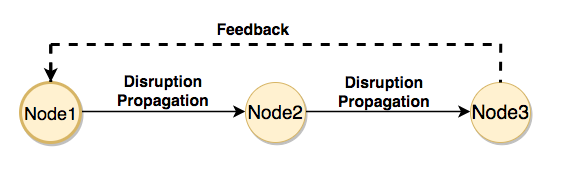
\includegraphics[width=4.0in]{figures/pdf/Cyclical-Linkage.png}\\
  \caption{Cyclical Linkage Representation}\label{Cyclical Linkage}
\end{figure}


The disruptions occurring in the cyclical linkages are the most underestimated in the entire supply chain. But, these have a very significant impact on the supply chain. These linkages should be considered from all the perspectives. There exists different cyclical linkages between different levels of the supply chain. There is a customer order cycle between the customer and the retailer; a replenishment cycle between the retailer and the distributor; a manufacturing cycle between distributor and the manufacturer; a procurement cycle between the manufacturer and the supplier. Any disruption in one of these cycles can lead to the disruption of the whole supply chain. 

The customer order cycle consists of 4 distinctive activities. These are customer arrival, customer order entry, customer order fulfillment, and customer order receiving. The replenishment cycle consists of retail order trigger, retail order entry, retail order fulfillment, and retail order receiving. The manufacturing cycle consists of order arrival, production scheduling, manufacturing and shipping, and receiving. The procurement cycle consists of order based on manufacturer's production schedule or supplier's stocking method, supplier production scheduling, component manufacturing and shipping, and receiving at manufacturer.



\newpage
\section{Network Structure}

(\citeauthor{Kim2015}, \citeyear{Kim2015}) have considered the network structural perspective for the supply network disruption and resilience. It can be inferred that in a network, the prime cause of interruption of the movement of the unit is the malfunction in the node or arc. Although it is the prime reason for the cause of interruption, it does not help in detecting the network-level disruption. In this paper, the methodology that has been used for the purpose of designing the supply chain network is the graph theory. It has been applied to a great extent to the complex networks like the World Wide Web, power grids, and the food chains (\citeauthor{gross2005graph}, \citeyear{gross2005graph}). If we implement the graph theory in the field of supply chain, then the facilities would be a representation of the nodes, whereas, the logistics between the facilities would be represented by the arcs.

\begin{figure}[H]
  \centering
  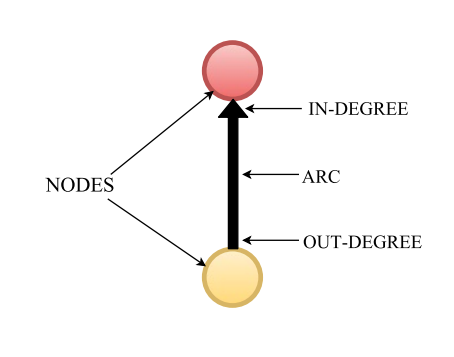
\includegraphics[width=2.5in]{figures/pdf/Node-structure.png}\\
  \caption{The structure of nodes and arcs according to the graph theory.}\label{Node structure}
\end{figure}


The latent structure of a supply chain network can be explained by the graph theory in a suitable manner. Instead of using the notations G = (V, E) (\citeauthor{emden1997complexity}, \citeyear{emden1997complexity}) ,the notation G=(N, A) is used in terms of supply chain design (\citeauthor{Kim2015}, \citeyear{Kim2015}). The set N contains the nodes while the set A contains the arcs of the supply chain network. It glances at the correlation between the nodes and arcs at a structural level from a meticulous perspective. The in-degree and out-degree are the elements that describe the amount of the supplier and customer present in the node in consideration. The in-degree resembles the number of arcs whose head connects to a node, and the out-degree resembles the number of arcs whose tail connects to the node. 

In the event of an arc or node level disruption, it has been observed that the supply chain may still continue to function normally, as there exists multiple walks from the initial node to the final node. The disruption does not seem to be affecting the supply chain network, since the materials are being delivered to their required final point from its initial point. But, the network level disruption can cause the system to fail or the process to remain incomplete.

For determining the performance of the network structure, a theoretical framework is provided by the complex adaptive systems (CAS) theory (\citeauthor{Kim2015}, \citeyear{Kim2015}). According to this theory, the analytic frameworks have been developed for the better understanding of the correlations between all the elements within the system. It sheds light on how these correlations affect the overall performance of the system. The structures that have been taken into consideration in this research paper are the ones that take place in the real-life SC scenario. These are as following:


\begin{itemize}
    \item Block-diagonal network structures
    \item Scale-free network structures
    \item Centralized network structures
    \item Diagonal network structures
\end{itemize}

The block-diagonal network structure is the one in which the nodes are clumped up between the initial and final node, where there are connections within the clumps but not between the clumps. The scale-free network pattern exhibits a biased nature, where a certain few nodes have most of the connections, while most of the other nodes obtain the merest of connections. This type of network pattern has node degree distribution which is highly distorted and seems to follow a power-law or Pareto distribution. The centralized structure is an accurate illustration of highly central nodes. In this, the high-level suppliers assume authority as a representative of the customer firm in the design and development processes. The diagonal supply structure follows a certain pecking order in which the materials are moved only in one direction (from the lower-level nodes to the higher-level node). These network structures are as shown Fig \ref{BDNS}, Fig \ref{SFNS}, Fig \ref{CNS}, and Fig \ref{DNS}.

\begin{figure}[H]
  \centering
  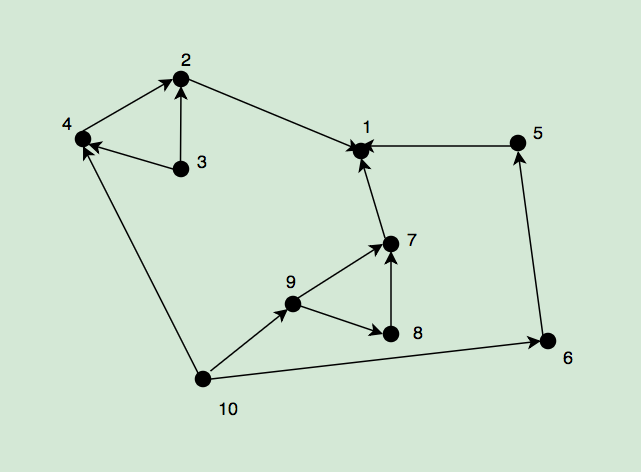
\includegraphics[width=4.5in]{figures/pdf/Block-diagonal.png}\\
  \caption{Block-Diagonal Network Structure} \label{BDNS}
\end{figure}

\begin{figure}[H]
  \centering
  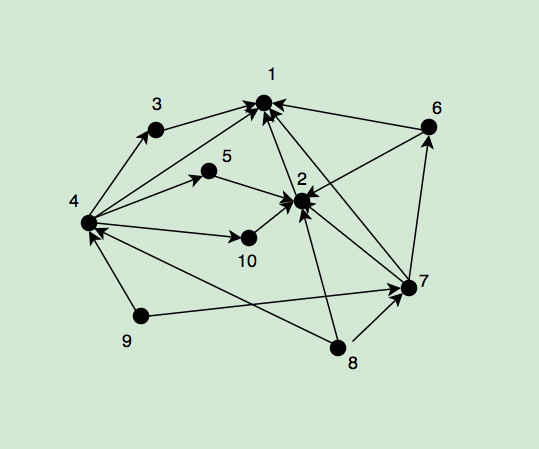
\includegraphics[width=4.5in]{figures/pdf/ScaleFree.png}\\
  \caption{Scale-free Network Structure} \label{SFNS}
\end{figure}

\begin{figure}[H]
  \centering
  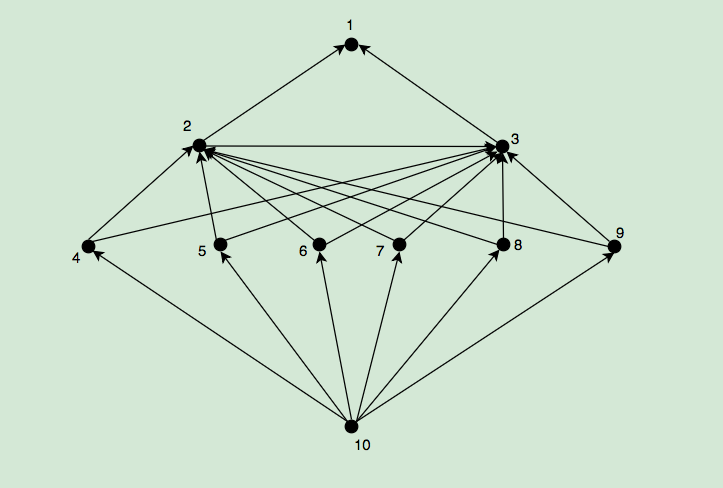
\includegraphics[width=4.5in]{figures/pdf/Centralized.png}\\
  \caption{Centralized Network Structure} \label{CNS}
\end{figure}

\begin{figure}[H]
  \centering
  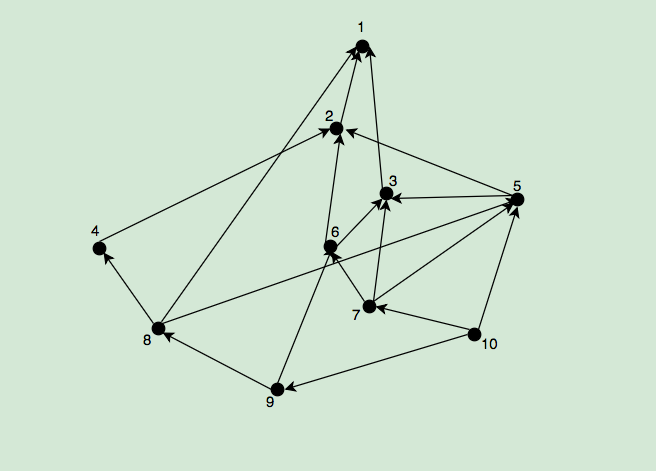
\includegraphics[width=4.5in]{figures/pdf/Diagonal.png}\\
  \caption{Diagonal Network Structure} \label{DNS}
\end{figure}

\newpage
For the evaluation of the best network structure, certain metrics are required to be defined and measured for all the structures. Based on these metrics, the resiliency of the structure can be determined. In this paper, the authors have defined and measured some resilience metrics that would be helpful in determining the resiliency of the network structures in consideration.

These resilience metrics are as follows:


\textbf{Network Density ($N_{\text{D}}$) :}
\begin{equation}
    N_D = \frac{N_T}{N_P}
\end{equation}
\newline
Where,
\newline
  $N_{\text{T}}$ = No. of total existing arcs
\newline  
 $N_{\text{P}}$ = No. of possible arcs
 

\textbf{Average In-Degree:} It is the mean of the number of arcs having their heads connected to the nodes throughout the network.

\textbf{Average Out-Degree:} It is the mean of the number of arcs having their tails connected to the nodes throughout the network.

\textbf{Connectivity:} It is the minimum number of nodes and/or arcs which when removed will disengage the network.

A supply network disruption occurs when the network is incomplete between the initial and final node due to the disruptions in the nodes/arcs. The supply network resilience can be determined by evaluating the probability that in case of a removal of a random node/arc between the nodes, then the network is still being completed between the initial and the final node.


Thus, the supply network resilience ($R_{\text{S}}$) can be written down mathematically as
\begin{equation}
   R_S = \frac{N_U}{N_D}
\end{equation}
Where,
\newline
$N_{\text{U}}$ = Total no. of node/arc disruptions, which do not lead to disruption
\newline
$N_{\text{D}}$ = Total no. of node/arc disruptions

On calculating and comparing these metrics for the structures that have been considered for the study, it is observed that the scale-free network structure has the highest score on the resilience index. It can be inferred from the calculations that the higher resilience does not necessarily come from the networks that are closely-packed or intricate. From the viewpoint of the network structures, a plethora of network does not yield an increase in resilience. In case of unanticipated disruptions, the network that has various tiers has a better chance of survival. The manner in which the nodes and arcs are connected to each other in a network influences the disruption risk and its resilience against the disruption.

Thus, from the aforementioned research it can be extrapolated that the network structure has a significant impact on the resiliency of the entire system. The resiliency of the supply chain network is impacted by the number of nodes and arcs it is made up of. The metrics such as network density, average in-degree, average out-degree, connectivity, and resilience can be further applied to the concepts of cyclical linkages and the correlation of risks in the supply chain. Thus, these two concepts can be further worked on for aiding the improvement of the resilience of the supply chain.


\section{Implementation of Simulation in Supply Chain Design} 
    
In today's world the nature of the supply chain has become very complex both in size and structure. There are multiple players and facilities present in them. Due to inter-connectivity and inter-dependencies present in them, the supply chains are prone to have disruptions that may disseminate throughout the network. If the supply chains are relatively small, then the uncertainties can be easily mitigated through the techniques of communication and managerial decisions due to the involvement of few players. On the other hand, if the supply chain is considerably large, then the same techniques would prove to be useless. A lot of significant information would be lost somewhere along the communication. Thus, there arises a need for using simulation software that provide an environment to model supply chains having any number of players and facilities and in real time. It is possible to model the supply chain at individual levels so that each player can be considered very carefully. This aids us in making modifications in the parameters at the individual level in the face of disruption, such that there is a sense of continuity maintained throughout the supply chain. Thus, making the supply chain resilient and robust. The simulation software helps us in quantifying our methodology. Alternate facility selection can be easily achieved through the simulation software. The facilities are selected in such a manner that they can fulfill the needs of the disrupted facility in less time and less cost. Simulation allows us the flexibility to work with different alternatives to resolve the impact of disruptions on the supply chain. It also helps us in understanding the ripple effect of disruptions and its impact throughout the supply chain.




    \chapter{Literature Review} \label{ch:litreview}

There has been quite a lot of research in the comprehension of the concepts of resiliency and robustness in the supply chain and its significance. Many firms have faced the adverse effects of disruption on the performance of their supply chains. The loss in terms of money, time, and the trust of the customers have forced the managers and owners to turn to the recourse of having resiliency and robustness incorporated in their initial design phase of the supply chain. 

The management of disruptions and the decisions that are made during the occurrence of a disruption plays a pivotal role in defining the performance and quality of the system. This can prove to have an advantage over the competitors. An example of this is the approach and decision-making skills of Nokia when the radio frequency chip manufacturing plant of Philips electronics was caught on fire. Even though the fire was contained and taken care of in less than 10 minutes, the effects of the fire had a heavy impact on the chips that were present in the storage area. Due to the water and smoke, the chips in the storage were damaged and rendered useless. Philips was a major chip suppler to Nokia and their competitors Ericsson. The Philips management declared to their customers (Nokia and Ericsson) that the disruption would be taken care of within the span of a week. While the management at Ericsson were unaware of the impact that this disruption would be causing to them, the management personnel at Nokia sensed that this disruption would be of longer duration than promised. They (Nokia management) forced the Philips management to provide them with alternate sourcing of the chips by other manufacturing plants owned by Philips. Thus, the demands at the Nokia were met. Meanwhile, Ericsson were still waiting for the parts to arrive from Philips. This loss in time proved crucial to Ericsson and they incurred tremendous losses. Due to the proactive decision making and identifying the implications of the disruption by the Nokia personnel, they achieved profit and the trust of customers over their rivals Ericsson. 

\citep{Fujimoto2011} has outlined the importance of having a resilient supply chain by mentioning the case of the 1995 earthquake in Japan. The earthquake had massive impacts on the supply chains of Toyota and other companies in the affected areas. During the disaster, many of the facilities and plants that comprised of the parts provider for brakes and audio parts were completely levelled. The restoration of these plants were going to take a very long time which meant the production of the vehicles were going to come to a halt. Rather than just waiting for the plants to get restored, Toyota deployed personnel to the aid of getting the plants back to its functioning ability. In the meantime they had also developed a team that would search for alternate suppliers so that the production of the vehicles could be resumed as quickly as possible. This proved to extremely beneficial for Toyota as they reduced the down time to a few days rather than weeks. Thus, resiliency was incorporated by Toyota in their supply chain for having the minimum losses and getting the production of vehicles get back to the original level. Due to this, the importance of having a resilient supply chain came into light and various companies have started taking the initiatives to impart it in their supply chains.

\citep{Falasca2008} have done a considerable amount of research in the assessment of supply chain resilience. They developed a supply chain and made it undergo certain disruptions to study the effect of disruptions and to design the countermeasures to reduce the ramifications of the disruption. They have regarded supply chain structure as a number nodes that are inter-connected to each other. They have expressed the aspects of node density, node complexity, and node criticality as the three pillars that define the supply chain structure. If the disruption occurs in any of these pillars of the supply chain, then the entire supply chain would tremble. They have also mentioned that disruptions are more likely to take place in the supply chains having a significant amount of critical nodes. The method of simulation has been suggested as a methodology to replicate the supply chain structure and to understand its behavior under disruption. The cause-effect analysis of the measures taken to make the supply chain resilient can be obtained through the use of simulation. This research is used as the foundation for using simulation as a methodology in our study. This research also signifies resilience during the event of disruption in a supply chain.

\citep{Li2018} have developed an agent-based simulation model which focuses on fortifying the facility within a supply chain during disruptions. They have made use of the p-median problem model for choosing the facility which has the least distance for transportation. The RIMF method has been used to select the protective resources at the lowest costs in order to have the least impact during the disruption. In their study, they have created a supply chain consisting of 100 demand points in the United States of America. Out of these 100, 20 demand points are chosen at random to act as the distributors.  There are two scenarios for the occurrence of disruptions which have been developed in this study. In the first scenario, the three most important distributors in the network are fortified based on their importance score. In the second scenario, the four most important distributors are fortified. Once the disruptions occur at the distributors and that facility is destroyed, the p-median and RIMF methods help in choosing the facility such that the distance travelled is as minimum as possible, and the recovery of the destroyed facility at the lowest costs incurred. The most noteworthy points to be taken from this study is the use of agent-based simulation to study the effect of disruptions on the supply chain, the most cost effective method to resolve the disruptions, and the alternate facility selection having the least distance travelled.

The importance of the resilience and robustness can be easily observed from the research papers. Also, the role that simulation software plays an important role in quantifying the significance of these two terms in supply chain by giving the visual representation of the supply chain under disruptive conditions. Thus, we have made use of agent-based simulation in our study.


    \chapter{Methodology}\label{ch:methodology}

In this study, we have considered the Agent-based simulation as our primary methodology for illustrating our supply chain model and accounting for disruptions. The supply chain model consists of 5 Suppliers, 7 Manufacturers, 10 Distributors, and 20 Retailers. Each facility acts as an individual agent which has been placed across the United States. The model represents the supply chain of one company having different facilities throughout the country. In the event of disruption, if any of the facilities gets shut down, then they have an alternative facility to turn to in order to get their demands satisfied. In the meantime, the facility that has been affected by the disruption is revived by taking the correct measures to increase the resiliency. Each facility has been assigned certain parameters of cost, time and demand fulfillment rate. There is a constant flow of materials downwards through the agents in the supply chain, while there is a constant flow of information upwards through the agents in the supply chain. It is important that this flow never breaks for the efficient performance of the system. In order to maintain this flow during disruption, alternate facilities are selected. The alternate facility gets selected based on the best parameter values amongst the available lists of facilities. There are a total of 5 scenarios depicting the source of disruption in the supply chain. The different strategies that need to be taken as per the source of the disruption are encompassed in the model for the purpose of restoration of the disrupted facility. The most efficient and appropriate strategy makes a massive impact on the resiliency of the system.


\newpage
\section{Agent-Based Modeling}

The main reason for developing the supply chain model as an agent-based simulation was due to the freedom to express the interaction between agents which is absolutely necessary to consider in our model. The complex nature of the supply chains makes it difficult to design models using the basic simulation models. Agent-based simulation helps in exhibiting the exact nature of a supply chain and all its players. The decision-making, information sharing, uncertainties, trade-offs, and coordination can be accurately represented by the agent-based simulation. It proves as the perfect platform to analyze different strategies and select the best one by implementing in the already existing model. The results are obtained at a fast rate and at an higher accuracy. 

\subsection{The Agents involved}

The model that we have developed for the purpose of our study contains four different agent types and are connected to each other for maintaining a sense of completion. Each agent type has a number of agents that are positioned across the United States of America. If the connections are lost, that means the supply chain has faced a disruption at some point in the network. The description of these agent types and the parameters associated with them are as follows.

\subsubsection{I. Supplier Agent}

These are the facilities that provide the raw materials to the manufacturing facility. In our model, there a total of 5 suppliers positioned across the country. The nomenclature for the suppliers has been done as S1, S2, S3, S4, and S5. The parameters associated with them are response time (time required to fulfill the demands of the manufacturer) and the raw material handling costs. The costs such as raw material handling cost and inventory holding costs are usually a percentage of the total costs. According to research, the percentage value for these costs lies between the range 40 to 60 percent of the total costs. The values of the parameters are as shown in the Table \ref{tab:Supplier}.

\begin{table}[H]
\caption{Parameters of the Supplier}
\label{tab:Supplier}
\begin{center}
\begin{tabular}[b]{|c|c|c|}
	\hline
	Supplier & Raw Material Handling Cost & Response Time \\ \hline
	S1 & 0.45 & High\\ \hline
	S2 & 0.52 & Medium \\ \hline
	S3 & 0.44 & High \\ \hline
	S4 & 0.58 & Low \\ \hline
	S5 & 0.56 & Medium \\ \hline
\end{tabular}
\end{center}
\end{table}

The values corresponding to the response time have ranking from 1 to 3. The rank 1 means that the response time is low, which is highly favorable for the selection criteria. Rank 2 and Rank 3 are the response time medium and high respectively. In the event of disruption, if a supplier is down, then alternate supplier is selected in such a way that the response time is either low or medium, and the raw material handling cost is the minimum.

\subsubsection{II. Manufacturer Agent}

Once the raw material has been acquired from the supplier, it comes to the manufacturer where it is converted into the final product. In our model, the 5 suppliers dispatch the raw materials to 7 manufacturers. These manufactures are positioned around the country and their nomenclature is done as M1, M2, M3,M4, M5, M6, and M7. The parameters associated with the manufacturer agents are inventory holding cost and response time. In the event of disruption, if any of the manufacturer that fulfills the demands of the distributors associated with it is down, then the alternate manufacturer is selected in such a way that the inventory holding cost is minimum, and the response time is either low or medium. The parameters for the manufacturer agent and their corresponding values are shown in the Table \ref{tab:Manufacturer}.


\begin{table}[H]
\caption{Parameters of the Manufacturer}
\label{tab:Manufacturer}
\begin{center}
\begin{tabular}[b]{|c|c|c|}
	\hline
	Manufacturer & Inventory Holding Cost & Response Time \\ \hline
	M1 & 0.51 & Low\\ \hline
	M2 & 0.41 & Medium \\ \hline
	M3 & 0.43 & Medium \\ \hline
	M4 & 0.57 & High \\ \hline
	M5 & 0.49 & Low \\ \hline
	M6 & 0.55 & High \\ \hline
	M7 & 0.48 & Low \\ \hline
\end{tabular}
\end{center}
\end{table}

\subsubsection{III. Distributor Agent}
The next agent is the distributor agent where the finished goods are collected from the manufacturer and are forwarded to the retailers. In our model we have 10 different distributors positioned across the country. The nomenclature for these 10 distributors is done as follows D1, D2, D3, D4, D5, D6, D7, D8, D9, and D10. The parameters associated with the distributors are inventory holding cost, order fulfillment rate, and response time. The selection of alternate distributor facility during disruption is done in such a way that the inventory holding cost should be minimum, order fulfillment rate should be high, and the response time should be low or medium. The parameters for the distributor agent and the values associated with them are as shown in the Table \ref{tab:Distributor}.


\begin{table}[H]
\caption{Parameters of the Distributor}
\label{tab:Distributor}
\begin{center}
\begin{tabular}[b]{|c|c|c|c|}
	\hline
	Distributor & Inventory Holding Cost & Order Fulfillment Rate & Response Time \\ \hline
	D1 & 0.46 & High & Medium\\ \hline
	D2 & 0.51 & High & High \\ \hline
	D3 & 0.44 & Low & Low \\ \hline
	D4 & 0.52 & High & High \\ \hline
	D5 & 0.48 & Low & Medium \\ \hline
	D6 & 0.49 & Low & Low \\ \hline
	D7 & 0.57 & High & Low \\ \hline
    D8 & 0.41 & High & Medium \\ \hline
    D9 & 0.48 & High & High \\ \hline
    D10 & 0.53 & Low & Low \\ \hline
\end{tabular}
\end{center}
\end{table}

\subsubsection{IV. Retailer Agent}
The fourth and final agent in our simulation model is the retailer agent. The retailers accrue the finished products from the distributors depending on the market trends and demands in their respective regions. In our model, there are a total of 20 retailers placed regionally across the country. Some regions have multiple retailers because of the high volume demand of the product from the customers. The nomenclature for the retailers are R1, R2, R3, R4, R5, R6, R7, R8, R9, R10, R11, R12, R13, R14, R15, R16, R17, R18, R19, and R20. A number of different retailer agents are connected to the same distributor agent. The parameter associated with the retailer agent is the response time (to the customers). The values corresponding to this parameter for the retailer agent is as shown in the Table \ref{tab:Retailer}.

\begin{table}[H]
\caption{Parameters of the Retailer}
\label{tab:Retailer}
\begin{center}
\begin{tabular}[b]{|c|c|}
	\hline
	Retailer & Response Time \\ \hline
	R1 & Low \\ \hline
	R2 & Medium \\ \hline
	R3 & Low \\ \hline
	R4 & High \\ \hline
	R5 & High \\ \hline
	R6 & Medium \\ \hline
	R7 & High \\ \hline
	R8 & Low \\ \hline
	R9 & Low \\ \hline
	R10 & Medium \\ \hline
	R11 & High \\ \hline
	R12 & Low \\ \hline
	R13 & Medium \\ \hline
	R14 & Medium \\ \hline
	R15 & High \\ \hline
	R16 & High \\ \hline
	R17 & High \\ \hline
	R18 & Low \\ \hline
	R19 & High \\ \hline
	R20 & Medium \\ \hline
\end{tabular}
\end{center}
\end{table}

\subsection{The Base Model Connections}
The four agent types are connected to each other to form 5 supply chains in the different regions throughout the country for a company. In the base model, the connections of the agents is as shown in the Fig.\ref{Base}. It can be observed from the Fig.\ref{Base} that the distributor D1 is shared by three retailers R3, R5 and R15. If there is a disruption in the area of Oregon and the distributor D1 is down due to it, then the retailers R3, R5, and R15 have to select a different distributor facility. They will choose the distributors from D2 to D10 based on who has the best parameter values. Similarly, the distributor agents and manufacturer agents connect to the best available manufacturer agent and supplier agent respectively based on the parameters. In the meantime, the restoration of the disrupted facility is taking place using appropriate mitigation strategies. This is the basic working logic of the whole simulation model.

\begin{figure}[H]
  \centering
  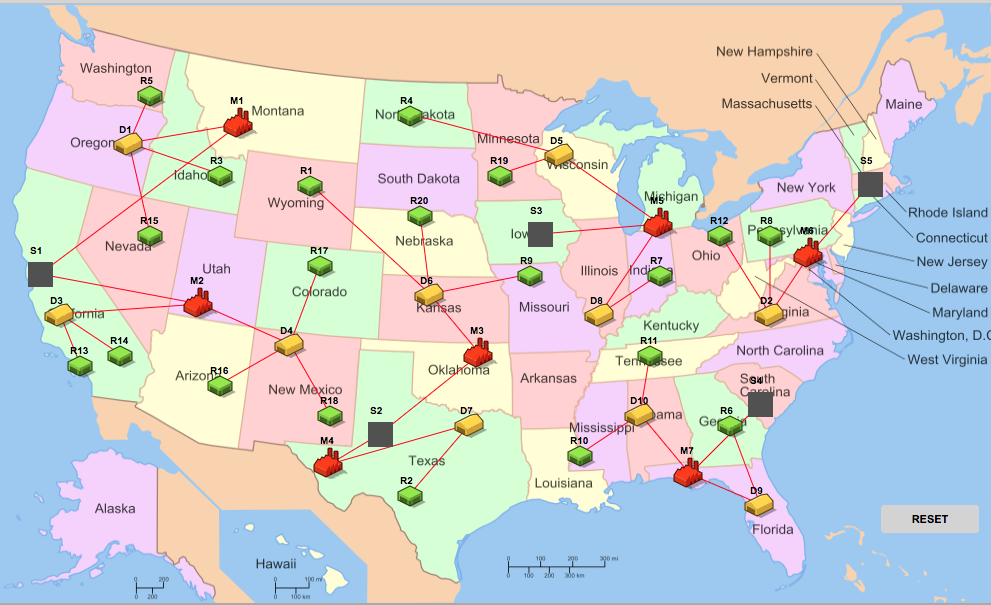
\includegraphics[width=6.5in]{figures/pdf/Basic-connections.png}\\
  \caption{Base Model Agent Connections.}\label{Base}
\end{figure}

\newpage
\section{Vulnerabilities and Capabilities}

There a lot of reasons for the disruptions to occur in the supply chain. Some may arise due to unfavorable natural conditions such as adverse weather, while some may be targeted attacks on firms. The knowledge of the source of disruption is very critical in order to devise proper mitigation strategies. If we know the reason of the disruption, then we can shift our focus on the repairing the most affected factors due to the disruption rather than doing the analysis of all the factors.

\begin{figure}[H]
  \centering
  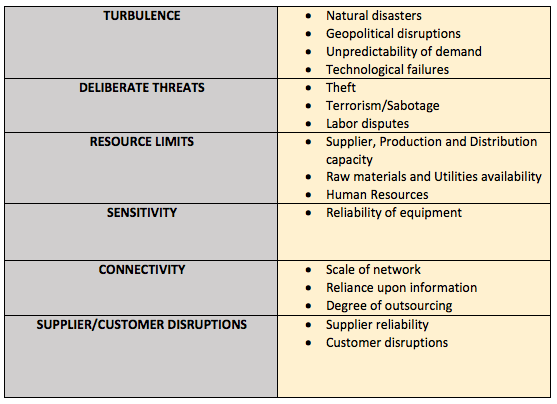
\includegraphics[width=6.0in]{figures/pdf/VNTS.png}\\
  \caption{Vulnerabilities and their various sources.}\label{Vulnerabilities}
\end{figure}

 \citep{Pettit2010} have jotted down these sources and factors as vulnerabilities and capabilities respectively. They have mentioned 7 vulnerabilities that lead to a disruption in the system. A firm should design its supply chain keeping in mind the relation between the vulnerabilities and capabilities. It should not have more capabilities as well as less capabilities. It should have just the perfect number of capabilities. If the company has enforced more capabilities, then there is a loss in capital. Also, if there are less capabilities, then the supply chain is left vulnerable to the disruptions.
 
We have implemented 6 out of the 7 vulnerabilities that act as a source of disruption. These vulnerabilities are as shown in the Fig.\ref{Vulnerabilities}. The major problem that occurs during resolving a disruption in a system is the time taken for thorough analysis of the root cause of the problem.

\begin{figure}[H]
  \centering
  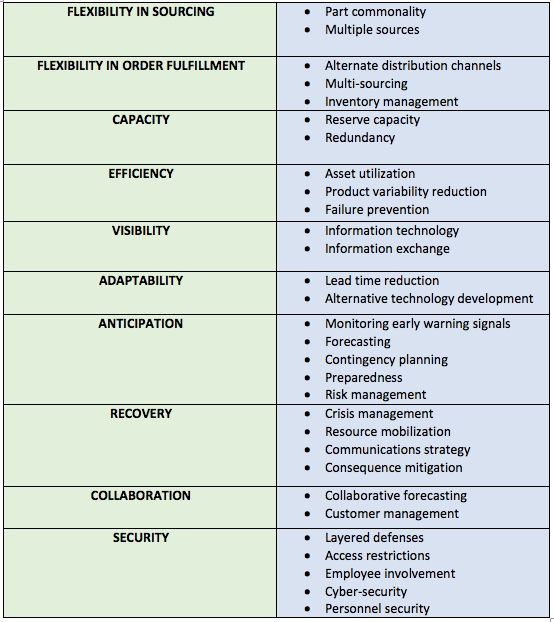
\includegraphics[width=6.0in]{figures/pdf/C1.png}\\
  \caption{Capabilities and their various types.}\label{Capabilities}
\end{figure}

 If the managers are well aware of the most common and recurring sources of disruption, they might be able to take preventive and reactive measures during disruptions of similar type in the future. By implementing these vulnerabilities in our supply chain design, we are not only providing ready measures of repair but also reducing the impact of disruption. Thus, making the system both resilient and robust in nature.  



\begin{figure}[H]
  \centering
  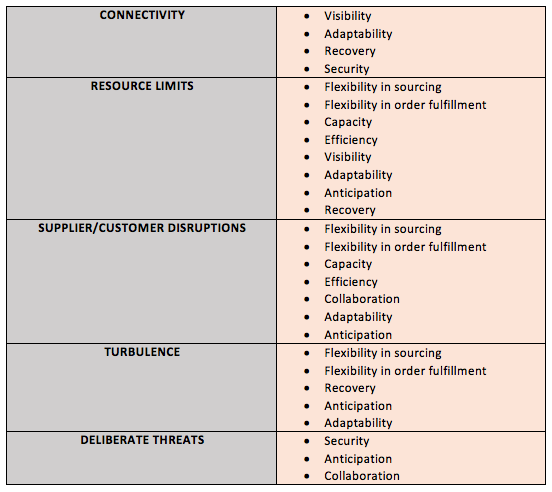
\includegraphics[width=6.0in]{figures/pdf/CV.png}\\
  \caption{Capabilities vs Vulnerabilities.}\label{CV}
\end{figure}


Once that the vulnerabilities are addressed, the next step is to glance at the capabilities (factors) that are most likely to be affected due to a certain kind of disruption rather looking at all the factors. This will help in reducing the time to find out where the exact problem lies. The list of capabilities that affect the performance of the supply chain system is as shown in Fig\ref{Capabilities}. These capabilities start to get damaged once the disruption occurs. The vulnerabilities that are closely associated with the capabilities are as shown in the Fig\ref{CV}. These prove to be beneficial in identifying the key factors that can help in improving the speed of recovery of the system back to its functioning state.


\section{Scenarios in the model}
In a typical supply chain, disruption can occur at any of the levels. Thus, we have developed the scenarios in such a way that the disruptions are occurring at the distributor level, manufacturer level, and the supplier. Also, for all the three events, we have considered the scenarios in which the disruptions are occurring due to the vulnerabilities that have been mentioned earlier. In total, there are 18 different scenarios and three scenarios for the disruption modeling without considering for resiliency design to quantify the need for our study.

\begin{figure}[H]
  \centering
  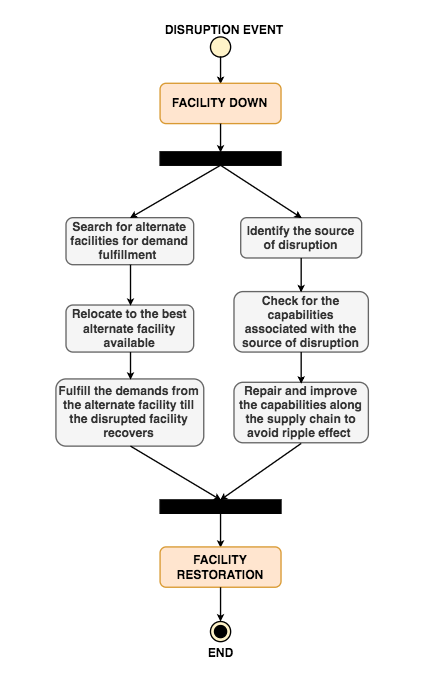
\includegraphics[width=2.0in]{figures/pdf/WL.png}\\
  \caption{Flowchart of Methodology.}\label{WL}
\end{figure}

 The working logic of the simulation model is as show in the Fig \ref{WL}. According to the logic, whenever the disruption occurs, the initial step is to identify the source of the disruption. The next step in the process is to check for the capabilities associated with the source of disruption that is most likely to get affected. During a disruption, it is not necessary that all the capabilities get damaged. Only a certain few capabilities get damaged which hinder with the performance of the system. The final step is to revive those damaged capabilities for getting the system functioning again.
 
The time between the occurrence of disruption and the identification of the key factors is called as the lost time ($T_{\text{L}}$). The time between the identification of the key factors and the total recovery of the disrupted facility is called as the recovery time $T_{\text{R}}$. The ratio of the recovery time to the lost time yields the resiliency percentage ($R_{\text{S}}$)  of the supply chain. 
 
 \begin{equation}
    Resiliency(R_S) = \frac{T_R}{T_L} \label{3.1}
\end{equation}

The higher the value of the resiliency, lesser is the length of recovery of the supply chain during disruption.

\subsection{Modeling without Resiliency and Robustness Consideration}
 In this model, the connections of the supply chain are as shown in the Fig\ref{Base}. There are three scenarios that can be observed for the behavior of supply chain under disruption. These scenarios are disruption at the distributor level, disruption at the manufacturer level, and disruption at the supplier level. Due to the absence of the key factor identification process in this model, a lot of time is wasted in finding out which factor of the supply chain is damaged which is hampering the entire system. Thus, the resiliency of the supply chain is going to have a lower value. 
 \subsubsection{Distributor Level Disruption}
 
 In this scenario, we have disrupted the distributor D3 which is located in the state of California. As the distributor D3 is down, it affects the other facilities associated with it. As a result, the demands from R13 and R14 retailers are not satisfied. A major backlog is recorder at these retailers due to the inability of those retailers to satisfy the customers in that area. The manufacturer M2 associated with the distributor D3 has to hold the inventory that was supposed to be delivered to the distributor. As the manufacturer is unaware of the duration of the recovery, it does not order any raw materials that were needed to manufacture the products that was supposed to be provided to the distributor. 
 
 \begin{figure}[H]
   \centering
    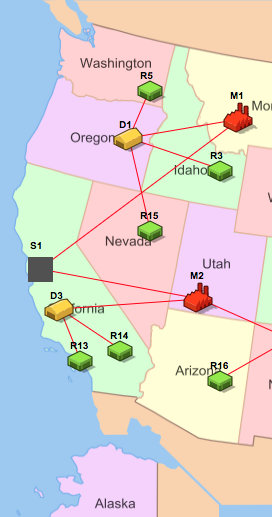
\includegraphics[width=1.5in]{figures/pdf/BeforeD.png} 
     \caption{Distributor Level Disruption (Before).}
     \label{fig:DLDb}
 \end{figure}
 
 \begin{figure}[H]
  \centering
  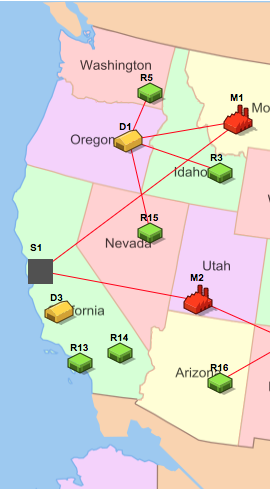
\includegraphics[width=1.5in]{figures/pdf/AfterD.png}
   \caption{Distributor Level Disruption (After).}
   \label{fig:DLDa}
\end{figure}

The connections before and after the disruption at the distributor D3 are shown in the Fig \ref{fig:DLDb} and Fig \ref{fig:DLDa}. It is evident from the figure that the disruption at the distributor causes D3 to disconnect from R13 and R14 retailers as well as M2 manufacturer.

\subsubsection{Manufacturer Level Disruptions}

In this scenario, we have disrupted the manufacturer M2 which is located in the state of Utah. As the manufacturer M2 is down, the effects of disruption spread throughout the supply chain through the facilities linked with it. As M2 is the manufacturer for two distributors D3 and D4, the two distributors are unable to collect the finished goods. As a result, the retailers R13, R14, R16, R17, and R18 are unable to fulfill the demands of the customers in their region. Thus, a backlog takes place both at the retailers and distributors. The supplier S1 linked to M2 has to hold the excess raw materials at their facility due to the uncertain duration of recovery of the disrupted facility. 

 \begin{figure}[H]
   \centering
    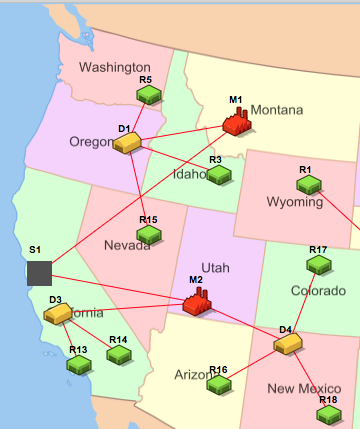
\includegraphics[width=2.0in]{figures/pdf/BeforeM.png} 
    \caption{Manufacturer Level Disruption (Before).}
    \label{fig:MLDb}
\end{figure}

\begin{figure}[H]
    \centering
   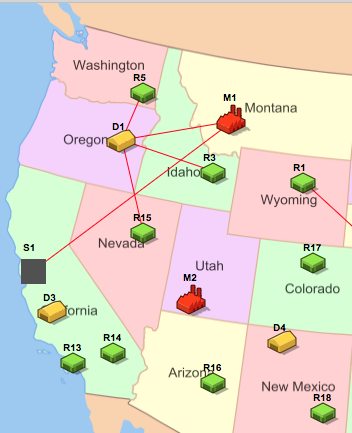
\includegraphics[width=2.0in]{figures/pdf/AfterM.png}
   \caption{Manufacturer Level Disruption (After).}
   \label{fig:MLDa}
\end{figure}

The connections before and after the disruption at M2 are shown in the Fig \ref{fig:MLDb} and Fig \ref{fig:MLDa}. The disruption causes the facilities R13, R14, R16, R17, R18, D3, and D4 to become inactive. The supplier S1 gets disconnected from the manufacturer M2.

\subsubsection{Supplier Level Disruption}

In this scenario, we disrupt the supplier facility S1 which is located in the state of California. Due to this, all the facilities that are linked to it get disrupted in one way or the other. The supplier S1 is the main and only provider of raw materials to the manufacturers M1 and M2. Thus the distributors and retailers associated with these two manufacturers have to wait for the S1 facility to recover from the disruption and provide the goods to the manufacturers so that they would be able to procure it from the manufacturers. 

\begin{figure}[H]
  \centering
  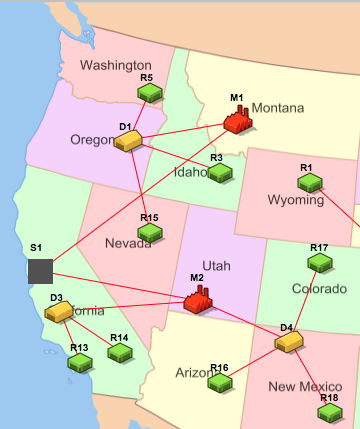
\includegraphics[width=2.5in]{figures/pdf/BeforeS.png}\\
  \caption{Supplier Level Disruption (Before).}\label{SLDB}
\end{figure}

\begin{figure}[H]
  \centering
  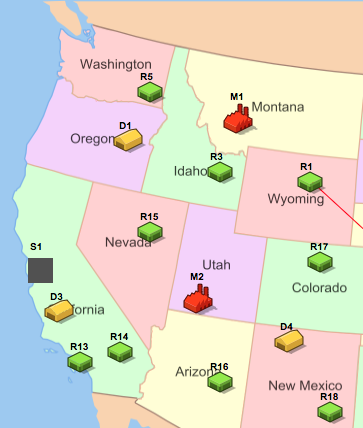
\includegraphics[width=2.5in]{figures/pdf/AfterS.png}\\
  \caption{Supplier Level Disruption (After).}\label{SLDA}
\end{figure}

In the Fig\ref{SLDB} the connections before the disruption at the supplier level are shown. The Fig\ref{SLDA} shows the disconnections caused due to the disruption at the supplier level. The facilities M1, M2, D1, D3, D4, R3, R5, R13, R14, R15, R16, R17 and R18 become inactive as they wait for the supplier S1 to recover from the disruption.

The lost time and recovery time occurred during different scenarios has a different value. Apart from the loss of time, there are other ramifications such as the backlog cost, inventory holding cost and the loss of customer loyalty. In this model the distributor level disruption causes a delay of a duration of 2 days. Out of this duration, the time for recovery ($T_{\text{R}}$) consisted of 12 hours while the lost time ($T_{\text{L}}$) was 36 hours. The resiliency of the model in this scenario is calculated as

\begin{equation}
    Resiliency(R_S) = \frac{12}{36} = 33.33 \% \label{3.2}
\end{equation}

The disruption at the manufacturer level causes a delay of 4 days in the supply chain. Out of these 4 days, the recovery time ($T_{\text{R}}$) is of 18 hours. The lost time ($T_{\text{L}}$) in this scenario is 78 hours. Thus, the resiliency of this scenario is even lesser than the previous scenario. It is calculated as

\begin{equation}
    Resiliency(R_S) = \frac{18}{78} = 23.07 \% \label{3.3}
\end{equation}

The disruption in the supplier level causes a delay of a week in the entire supply chain. The time for recovery ($T_{\text{R}}$) in this scenario is 24 hours, while the lost time ($T_{\text{L}}$) in this scenario is 144 hours. The resiliency of this scenario is calculated as

\begin{equation}
    Resiliency(R_S) = \frac{24}{144} = 16.66 \% \label{3.4}
\end{equation}

Among the three, the retailer level disruption scenario seems to have a better resilience value due to short difference of time between the lost time and the recovery time. It is to be noted that the duration of the disruption as well as the recovery time and lost time have been assumed. These values have been assumed so that the importance of implementing resilience and robustness in the supply chain can be quantified. There can be a huge variation in these values depending on the source of disruption. The values of resiliency obtained from the equations \ref{3.2}, \ref{3.3}, and \ref{3.4} are the values obtained during the disruption due to turbulence. Similarly, the values for resiliency of the system under different disruption sources can be obtained. The time lost ($T_{\text{L}}$) during these scenarios remains at all levels are the similar to that of the disruption due to turbulence. Thus the resiliency values for the other vulnerabilities that we have considered can be found out as well.

\subsubsection{Resiliency under disruption due to vulnerability due to Supplier/Customer Disruptions:}

\textit{At Distributor Level}
\begin{equation}
    Resiliency(R_S) = \frac{8}{36} = 22.22 \% \label{3.5}
\end{equation}
\newline
\textit{At Manufacturer Level}
\begin{equation}
    Resiliency(R_S) = \frac{14}{78} = 17.94 \% \label{3.6}
\end{equation}
\newline
\textit{At Supplier Level}
\begin{equation}
    Resiliency(R_S) = \frac{20}{144} = 13.88 \% \label{3.7}
\end{equation}

\subsubsection{Resiliency under disruption due to vulnerability due to Resource Limits:}

\textit{At Distributor Level}
\begin{equation}
    Resiliency(R_S) = \frac{6}{36} = 16.67 \% \label{3.8}
\end{equation}
\newline
\textit{At Manufacturer Level}
\begin{equation}
    Resiliency(R_S) = \frac{12}{78} = 15.38 \% \label{3.9}
\end{equation}
\newline
\textit{At Supplier Level}
\begin{equation}
    Resiliency(R_S) = \frac{18}{144} = 12.5 \% \label{3.10}
\end{equation}

\subsubsection{Resiliency under disruption due to vulnerability due to Connectivity:}

\textit{At Distributor Level}
\begin{equation}
    Resiliency(R_S) = \frac{11}{36} = 30.56 \% \label{3.11}
\end{equation}
\newline
\textit{At Manufacturer Level}
\begin{equation}
    Resiliency(R_S) = \frac{17}{78} = 21.79 \% \label{3.12}
\end{equation}
\newline
\textit{At Supplier Level}
\begin{equation}
    Resiliency(R_S) = \frac{23}{144} = 15.97 \% \label{3.13}
\end{equation}

\subsubsection{Resiliency under disruption due to vulnerability due to Deliberate Threats:}

\textit{At Distributor Level}
\begin{equation}
    Resiliency(R_S) = \frac{10}{36} = 27.78 \% \label{3.14}
\end{equation}
\newline
\textit{At Manufacturer Level}
\begin{equation}
    Resiliency(R_S) = \frac{16}{78} = 20.51 \% \label{3.15}
\end{equation}
\newline
\textit{At Supplier Level}
\begin{equation}
    Resiliency(R_S) = \frac{22}{144} = 15.27 \% \label{3.16}
\end{equation}


Thus, there arises a need for designing a supply chain with resilience and robustness incorporated in it as there is a huge scope in reducing the time lost in recognizing the key indicators of the system. 


\subsection{Modeling with Resiliency and Robustness Consideration}

In this model, we have implemented the key indicator identification and contingency planning components into our supply chain. Whenever a disruption takes place, the source of the disruption is identified and a team of management personnel look into the capabilities that are most probable of being affected. In the meantime, an alternate facility having the lowest costs, high fulfillment rate, and low response time is selected from the other available facilities. There is transportation cost that is incurred due to alternate facility location. But, this cost is just a small price to pay in order to avoid huge losses if we wait for the damaged facility to be repaired. The lost time is reduced by a drastic amount and thus the total delay caused by the disruption is reduced while keeping the supply chain working simultaneously. Thus, a resilient and robust supply chain is achieved.

\subsubsection{SCENARIO I: Disruptions due to Turbulence}

In this scenario we have identified the source of disruption as turbulence. Theses disruptions are mainly caused by natural disasters, geopolitical disruptions, unpredictability of demand, and technological failures. As the source of disruption is identified, the capabilities associated can be inspected for the damages and the process of repairing the damages can be initiated for getting a rapid recovery. The key indicators identified during this type of disruption are flexibility in sourcing, flexibility in order fulfillment, recovery, anticipation, and adaptability. The disrupted facilities are the same as the previous model for the sole reason of comparison of the values obtained in the resiliency. Thus, signifying the need for resiliency and robustness in the supply chain design.

\subsubsection{Distributor Level Disruption}
In this part of scenario I, we are targeting the distributor D3 in the state of California. The moment the distributor D3 is down due to the disruption, with the help of contingency planning, an alternate distributor is selected for fulfilling the demands of the retailers R13 and R14. Thus, the supply chain has a continuous functionality. As we the source of the disruption is comprehended, the problems are identified much quicker. The recovery time also becomes lesser as we have the knowledge of what strategies need to be considered for improving the capabilities. Thus, the total down time of the facility is reduced by a substantial amount.

\begin{figure}[H]
  \centering
  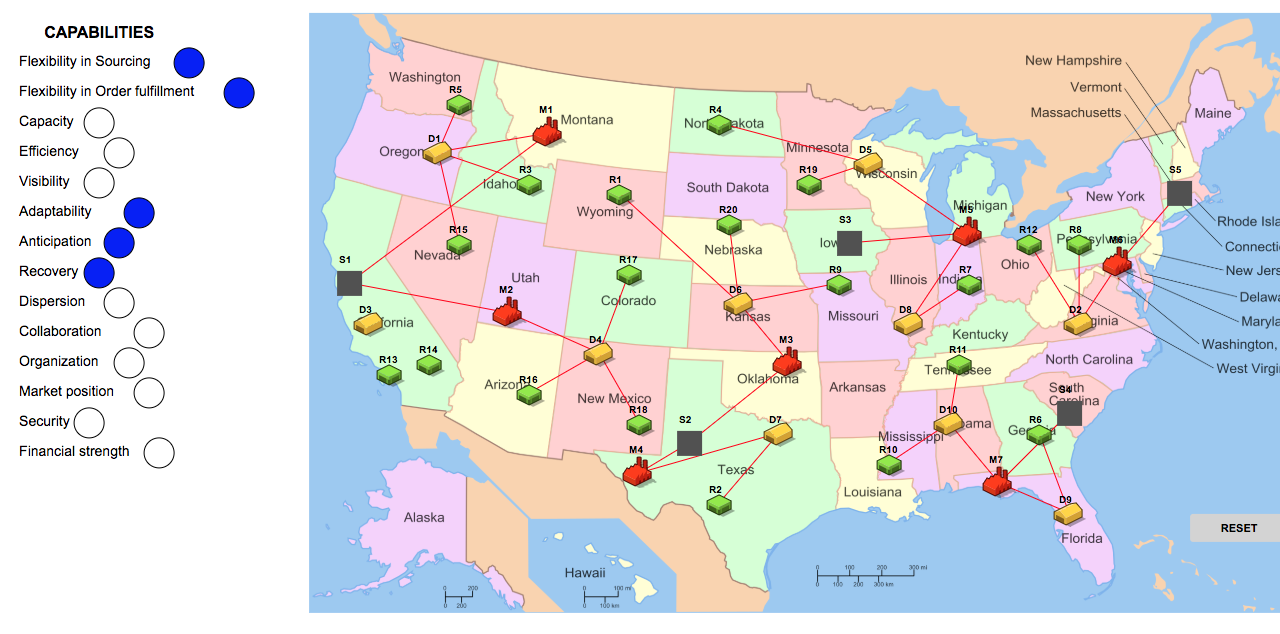
\includegraphics[width=6.5in]{figures/pdf/Scenario1DLD.png}\\
  \caption{Scenario I (Distributor Level Disruption).}
  {The distributor D3 is getting disrupted due to which the retailers associated with it are left unsatisfied. The manufacturer facility M2 is holding the inventory required by the disrupted facility D3. The capabilities associated with this type of disruption are being identified.}
  \label{SID}
\end{figure}

The Fig \ref{SID} shows the disrupted distributor D3 and the loss of its connection with the manufacturer M2, retailer R13, and retailer R14. The key indicators being identified can also be observed in this figure. The alternate distributor facility are selected for the retailers R13 and R14. There are three options that are selected by the simulation after putting the constraints as low or medium response time, high fulfillment rate, and minimum inventory holding cost. These distributor facilities are D1, D7 and D8 and the connections of the retailers R13 and R14 are as show in the Fig \ref{ALTD}. Out of these options, D1 is the best choice due to the proximity to the retailers. The transportation cost incurred would be lesser than the other two facilities.                                                            

\begin{figure}[H]
  \centering
  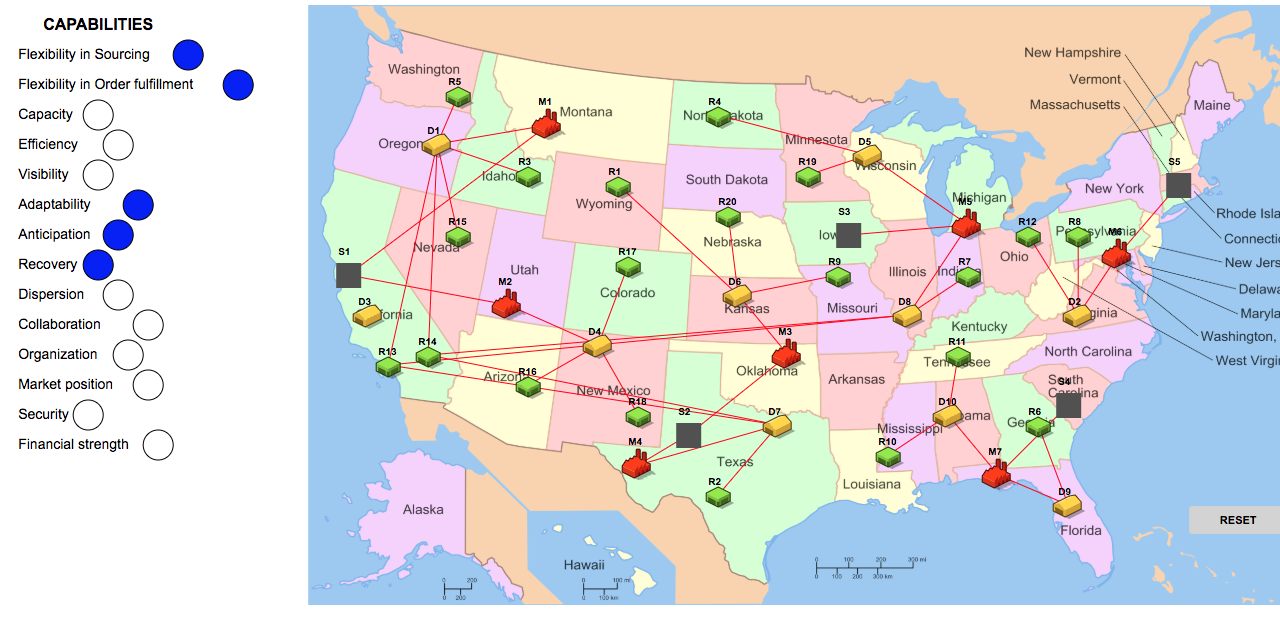
\includegraphics[width=6.5in]{figures/pdf/ALTD.png}\\
  \caption{Alternate Distributor Facility Selection Options for R13 and R14 retailers.}
  {The alternate distributor facilities D1, D7 and D8 are being selected as the possible options for the retailers R13 and R14 to maintain the continuous functioning state of the supply chain.}
  \label{ALTD}
\end{figure}                                                                                                            The lost time ($T_{\text{L}}$)  that is recorder in this scenario has been reduced to 18 hours due to the implementation of identification technique and contingency planning. The time for recovery ($T_{\text{R}}$) remains the same as 12 hours. Thus, the resiliency of the model appears to be having a higher value.

\begin{equation}
    Resiliency(R_S) = \frac{12}{18} = 66.67 \% \label{3.17}
\end{equation}

In this scenario, due to the contingency planning, the down time of the distributor does not cause any hampering effects on the other facilities associated with it. This is due to the retailers associated with the disrupted facility are allocated a different distributor that has the capability to fulfill their demands. However, the manufacturer facility M2 has to wait for the distributor D3 to be repaired. But, the waiting time is reduced in this scenario. Thus, the inventory holding cost will not be as much as in the scenario without resiliency consideration. Once the disrupted facility is repaired, the network gets back to its original state as shown in Fig \ref{Base}. 


\subsubsection{Manufacturer Level Disruption}

In this part of scenario I, an event is created where the manufacturer facility M2 is disrupted. The distributors associated with this facility disconnect from M2. The retailers connected to those distributors become inactive due to the disruption. The contingency planning comes into action here and the distributors D3 and D4 are relocated to other available manufacturers. Their retailers become active once they get relocated to different facilities. The effect of the manufacturer level disruption on the supply chain is as shown in the Fig \ref{S1MLD}. 

\begin{figure}[H]
  \centering
  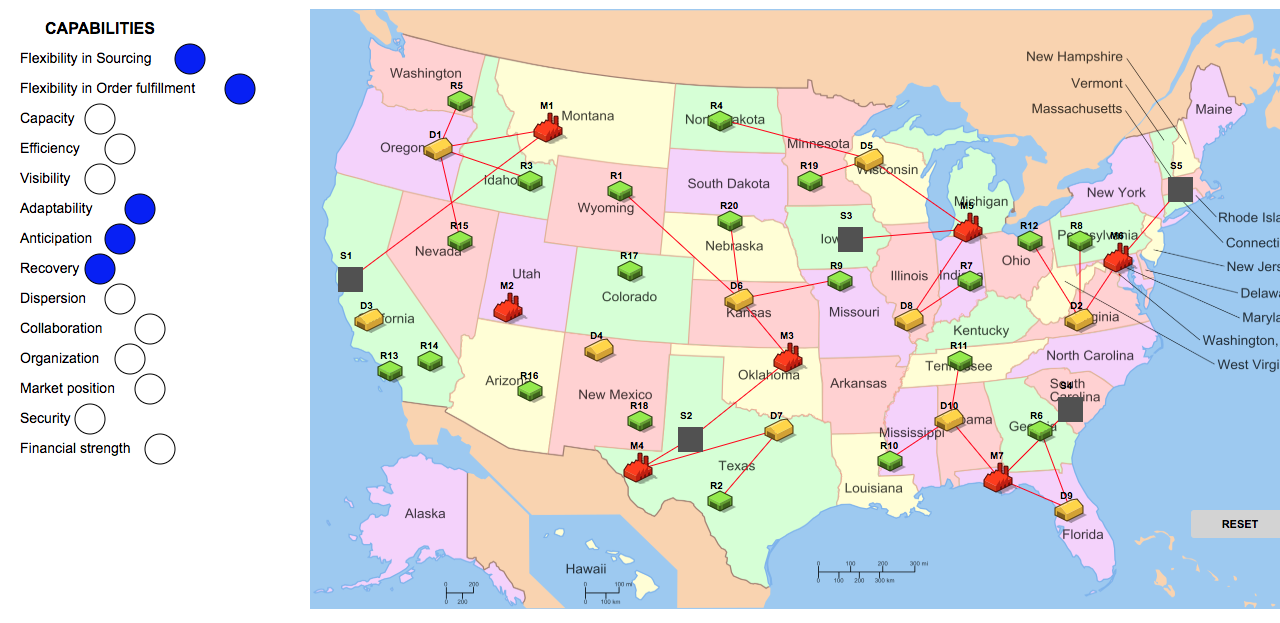
\includegraphics[width=6.5in]{figures/pdf/S1MLD.png}\\
  \caption{Scenario I (Manufacturer Level Disruption).}
  {The manufacturer M2 is getting disrupted due to which the  distributors and retailers associated with it are left unsatisfied. The supplier facility S1 is holding the inventory required by the disrupted facility M2. The capabilities associated with this type of disruption are being identified.}
  \label{S1MLD}
\end{figure}    

Through the contingency planning, the simulation software selects three options available for the relocation of the distributors D3 and D4. These selections are based on the constraints of low inventory holding cost and  low/medium response time. These manufacturing facilities are M3, M5, and M7 and are as shown in the Fig \ref{ALTM}. Out of these alternatives, the facility M3 has an advantage over the others in terms if inventory holding cost and transportation cost. 

\begin{figure}[H]
  \centering
  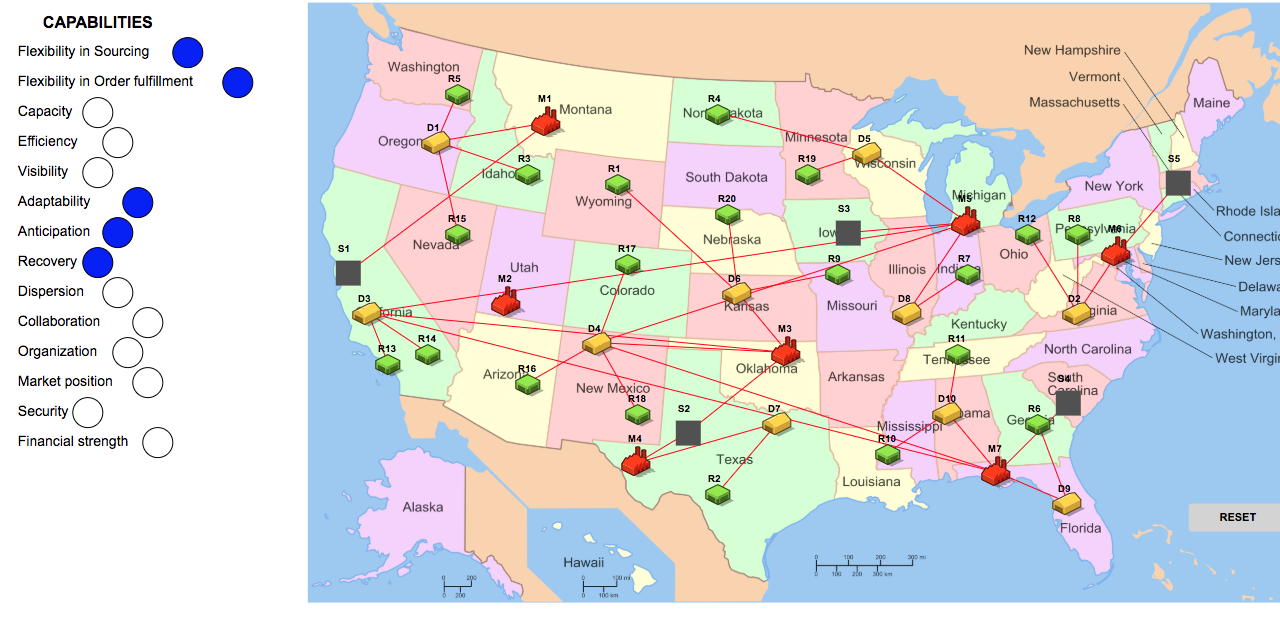
\includegraphics[width=6.5in]{figures/pdf/ALTM.png}\\
  \caption{Alternate Manufacturer Facility Selection Options for D3 and D4 distributors.}
  {The alternate manufacturer facilities M3, M5 and M7 are being selected as the possible options for the distributors D3 and D4 to maintain the continuous functioning state of the supply chain.}
  \label{ALTM}
\end{figure}    

During the alternate sourcing of the manufacturers for D3 and D4, the facility M2 is in the repairing process with the help of key indicator identifications. The lost time ($T_{\text{L}}$) is reduced as well due to these identification strategies and is now 54 hours instead of 78 hours. The recovery time ($T_{\text{R}}$) remains the same as it is dependent on the source of disruption. The resiliency of the supply chain in this scenario has increased due to the reduction in the lost time ($T_{\text{L}}$) in the system. 

\begin{equation}
    Resiliency(R_S) = \frac{18}{54} = 33.33 \% \label{3.18}
\end{equation}

The contingency planning does not allow any discontinuities to take place in the supply chain. The distributors fulfill their demands from the manufacturer M3 till the facility M2 recovers from the disruption. When M2 is fully recovered, the distributors go back to their original manufacturers. Thus, the supply chain gets back to its original functioning state. 

\newpage
\subsubsection{Supplier Level Disruption}

The supplier level disruption contains an event that destroys the facility S1 and all the facilities connected to them get disrupted as well. This scenario has the most damaging effect on the supply chain as it can get the entire system come to a standstill. The manufacturers M1 and M2 are disconnected and therefore the distributors D1, D3 and D4 are disconnected as well. As a result, the retailers associated with these distributors are unable to satisfy the customer demands in their region. The effect of the supplier level disruption and the key factors identification in the supply chain is as shown in the Fig \ref{S1SD}.

\begin{figure}[H]
  \centering
  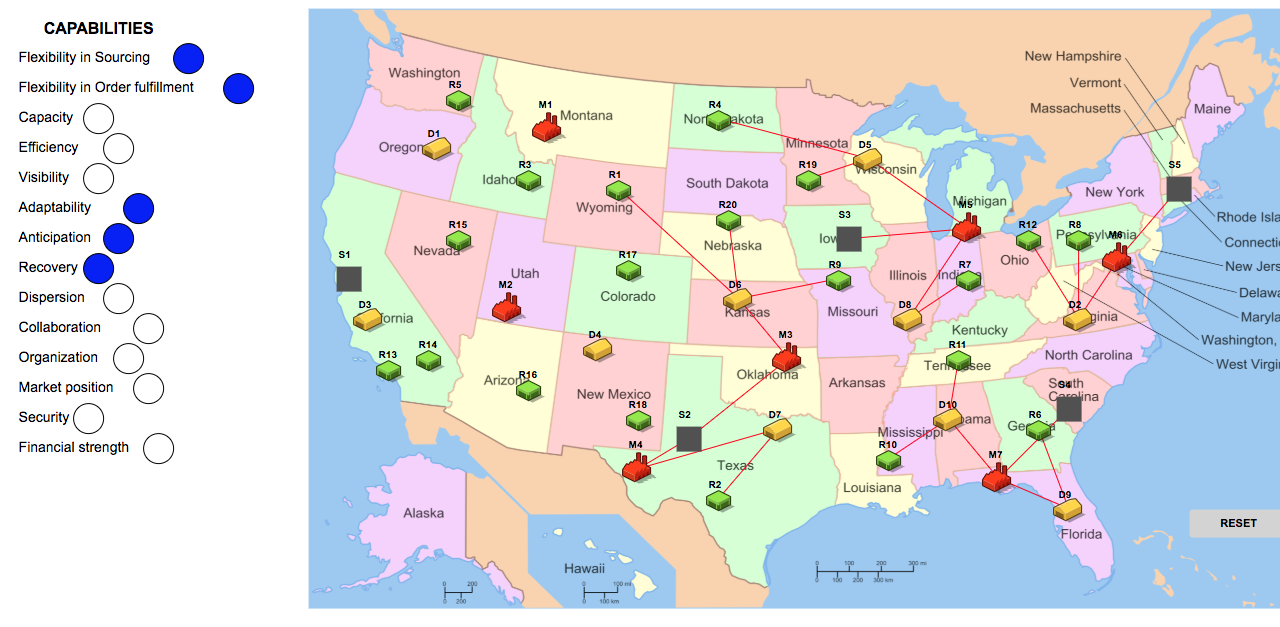
\includegraphics[width=6.5in]{figures/pdf/S1SLD.png}\\
  \caption{Scenario I (Supplier Level Disruption).}
   {The Supplier S1 is getting disrupted due to which the manufactures, distributors, and retailers are left unsatisfied. The entire supply chain is waiting for the facility S1 to be recovered for gaining back the functionality. The capabilities associated with this type of disruption are being identified.}
  \label{S1SD}
\end{figure}    

The entire supply chain gets disrupted when the S1 facility is disrupted. The key indicators are identified and the recovery process is initialized. With the help of contingency planning, the distributors are relocated to other available suppliers. The simulation tool aids us in finding the best supplier in terms of cost and response time. The constraints considered in the selection criteria are low raw material handling cost and low response time. There is only one supplier which meets the provided constraints. This supplier is the facility S4 and the alternate selection done by the simulation software is as shown in the Fig \ref{ALTS}.

\begin{figure}[H]
  \centering
  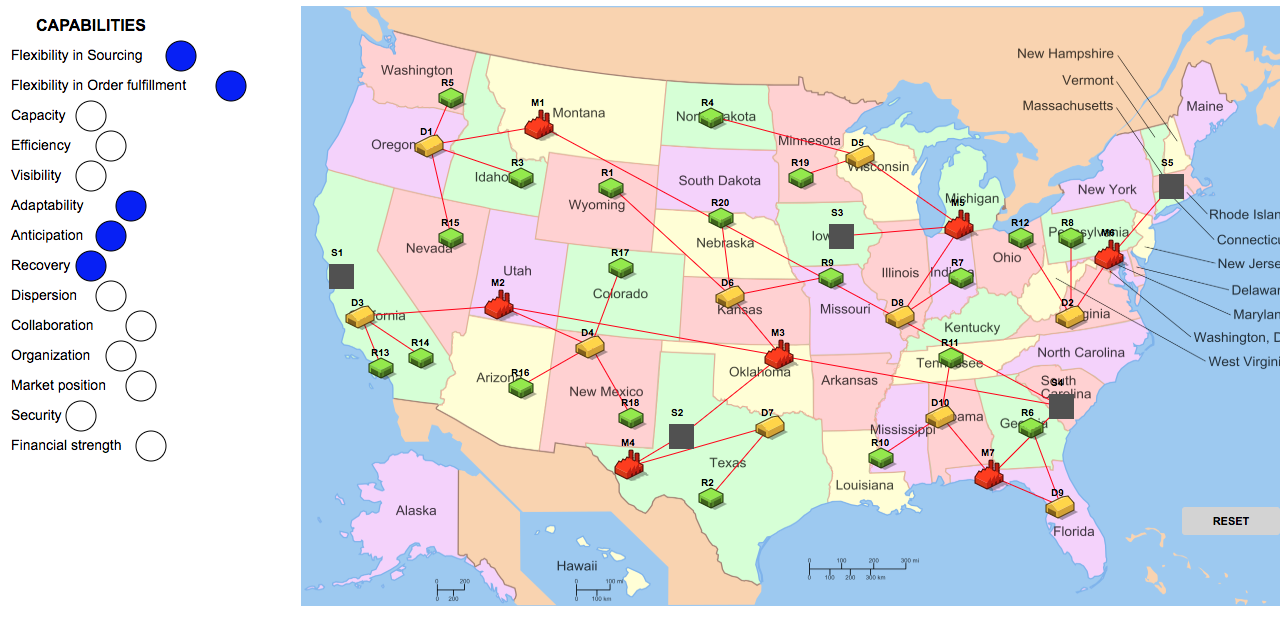
\includegraphics[width=6.5in]{figures/pdf/ALTS.png}\\
  \caption{Alternate Supplier Facility Selection Options for M1 and M2 manufacturers.}
  {The alternate supplier facility S4 is being selected for the manufacturers M1 and M2 to maintain the continuous functioning state of the supply chain.}
  \label{ALTS}
\end{figure}    

The manufacturing facilities M1 and M2 acquire the raw materials from the new supplier S4 till the disrupted facility S1 is recovered completely. Once the facility S1 is restored, the supply chain gets back to its original state.
The lost time ($T_{\text{L}}$) observed here is reduced by a huge amount to 96 hours from the original 144 hours. The recovery time still remains the same as the source of disruption is considered the same. The recovery time ($T_{\text{R}}$) value is 24 hours. The resiliency of the system is increased due to the reduction in the lost time. 

\begin{equation}
    Resiliency(R_S) = \frac{24}{96} = 25.00 \% \label{3.19}
\end{equation}

The inventory holding costs, loss of customer loyalty, and the backlog costs are eliminated due to incorporating the contingency planning and key indicators identification. Thus, the supply chain becomes resilient to disruptive events and becomes robust in the face of an uncertainty.

\newpage
\subsubsection{SCENARIO II: Supplier/Customer Disruptions}

This scenario encompasses the supplier/customer disruptions which occur very frequently. The main sources of this type of disruption are supply reliability and customer disruptions. Since we know the source of disruption, the key indicators (capabilities) are investigated and the recovery process can get underway. These key indicators are flexibility in sourcing, flexibility in order fulfillment, capacity, efficiency, collaboration, adaptability, and anticipation. Again, the disrupted facilities are kept same for the purpose of observing the performance of supply chain with and without contingency planning and key indicators identification. 

\subsubsection{Distributor Level Disruption}

\begin{figure}[H]
  \centering
  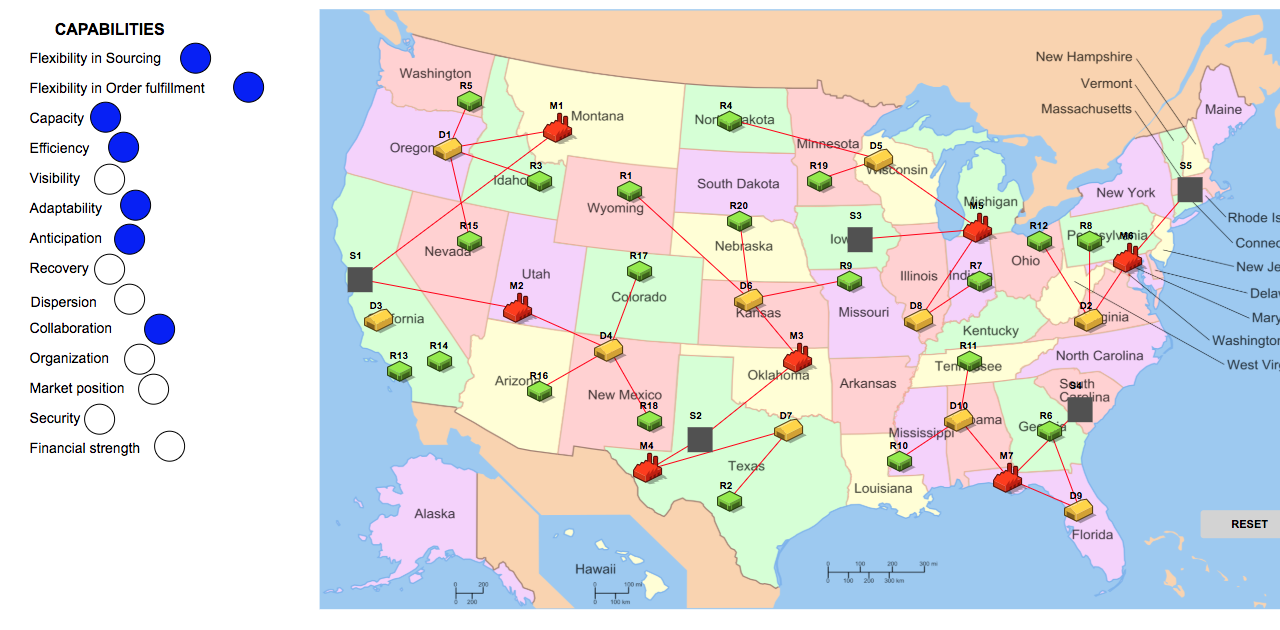
\includegraphics[width=6.5in]{figures/pdf/S2DLD.png}\\
  \caption{Scenario II (Distributor Level Disruption)}
  {The distributor D3 is getting disrupted due to which the retailers associated with it are left unsatisfied. The manufacturer facility M2 is holding the inventory required by the disrupted facility D3. The capabilities associated with this type of disruption are being identified.}
  \label{S2DL}
\end{figure}   

The Fig \ref{S2DL} shows the disruption occurring at the distributor level and the D3 facility is down. The retailers R13 and R14 along with the manufacturer M2 gets disconnected from D3. The cause of this uncertainty is the supplier/customer disruption and the key indicators associated with it are immediately addressed. The recovery process starts as soon as these capabilities are addressed. The alternate facility selection is the same as that of fig \ref{ALTD}. Thus, the lost time ($T_{\text{L}}$) is reduced due to the identification of the key capabilities. The time to recovery ($T_{\text{R}}$) remains the same as that of equation \ref{3.5}. The resiliency of this scenario is therefore increased.

\begin{equation}
    Resiliency(R_S) = \frac{8}{18} = 44.44 \% \label{3.20}
\end{equation}

By the introduction of contingency planning and key indicators identification into the supply chain design, the resiliency of supply chain was increased from 22.22 \% to 44.44 \% .

\subsubsection{Manufacturer Level Disruption}

\begin{figure}[H]
  \centering
  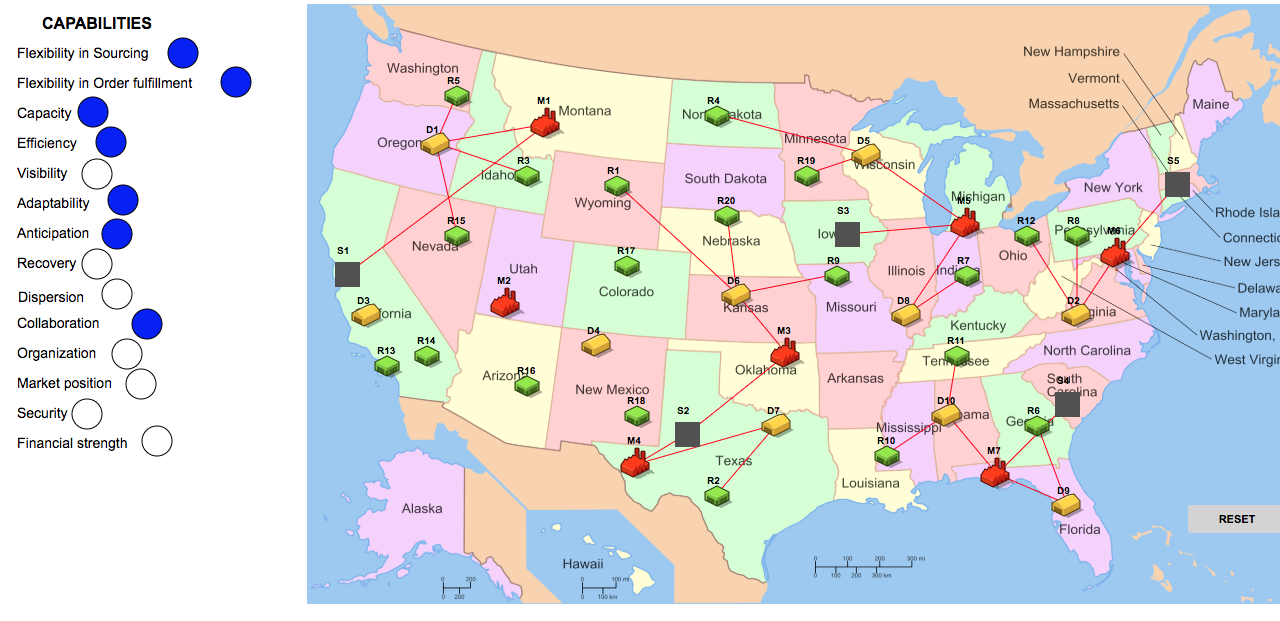
\includegraphics[width=6.5in]{figures/pdf/S2MLD.png}\\
  \caption{Scenario II (Manufacturer Level Disruption)}
  {The manufacturer M2 is getting disrupted due to which the  distributors and retailers associated with it are left unsatisfied. The supplier facility S1 is holding the inventory required by the disrupted facility M2. The capabilities associated with this type of disruption are being identified.}
  \label{S2ML}
\end{figure}   

The Fig \ref{S2ML} shows the disruption occurring at the manufacturer M2 causing the facilities D3, R13, R14, R16, R17, R18, D4 and S1 to disconnect from it. The raw materials are held up at the S1 facility till the facility M2 gets recovered, while the facilities D3 and D4 are inactive due to no supply of the materials to them. The identification of the key indicators help in resolving the issues caused due to the disruption at a faster rate. Thus, the lost time ($T_{\text{L}}$) is reduced while the recovery time ($T_{\text{R}}$) remains the same as that of equation\ref{3.6}. The resiliency of this system is comparatively better than that of the system without resiliency and robustness consideration. The contingency planning allocates an alternate manufacturing facility for D3 and D4 in the similar way as shown in Fig \ref{ALTM} till the M2 facility recovers. 

\begin{equation}
    Resiliency(R_S) = \frac{14}{54} = 25.92 \% \label{3.21}
\end{equation}

With the help of the resiliency and robustness consideration, the resiliency of the system in this scenario is increased from 17.94 \% to 25.92 \% .

\subsubsection{Supplier Level Disruption}

\begin{figure}[H]
  \centering
  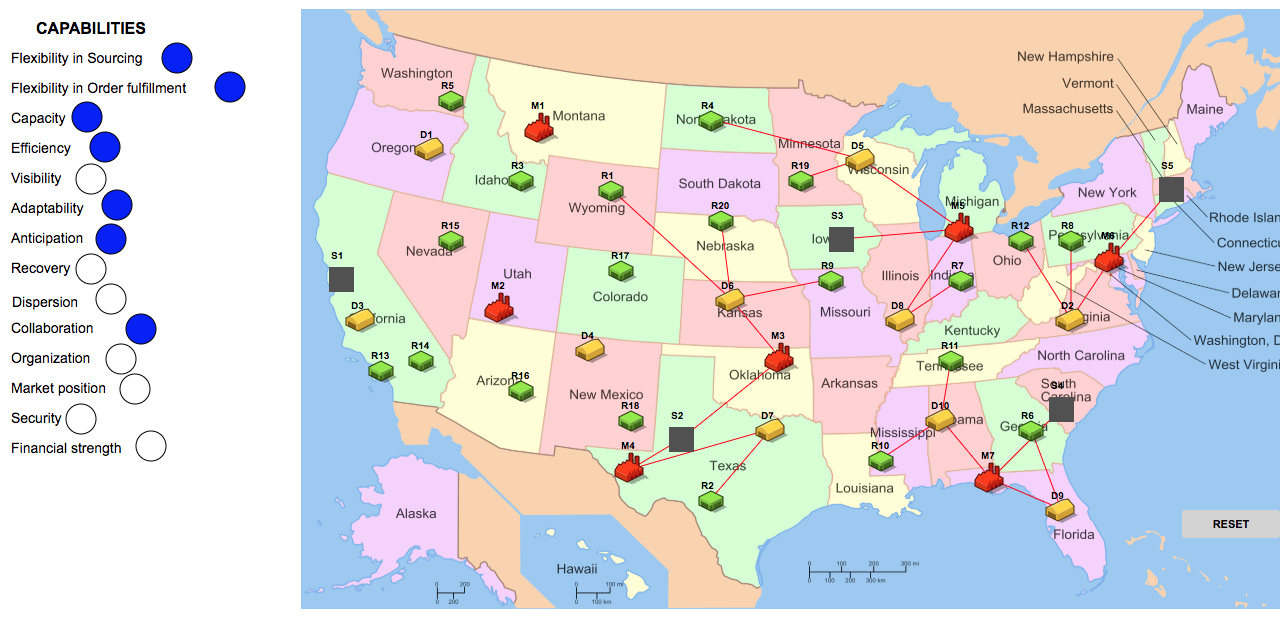
\includegraphics[width=6.5in]{figures/pdf/S2SLD.png}\\
  \caption{Scenario II (Supplier Level Disruption)}
   {The Supplier S1 is getting disrupted due to which the manufactures, distributors, and retailers are left unsatisfied. The entire supply chain is waiting for the facility S1 to be recovered for gaining back the functionality. The capabilities associated with this type of disruption are being identified.}
  \label{S2SL}
\end{figure}   

The Fig \ref{S2SL} shows the supplier facility S1 getting disrupted. The entire supply chain comes to a halt due to this disruption. The key indicators are identified and the recovery process is initiated. Thus, there is a need for alternate facility selection till the time the supplier S1 facility is recovering from the disruption. The contingency planning chooses alternate supplier facility for the manufacturers associated with S1 so that the supply chain maintains continuity. The new supplier is selected in the similar way as shown in Fig \ref{ALTS}. The recovery time ($T_{\text{R}}$) remains the same as that of equation \ref{3.7} while the lost time ($T_{\text{L}}$) is reduced due to the identification of key capabilities. The resilience of the system is thus improved.

\begin{equation}
    Resiliency(R_S) = \frac{20}{96} = 20.83 \% \label{3.22}
\end{equation}

The resiliency and robustness considerations increase the resilience of the supply chain from 13.88 \% to 20.83 \% .

\subsubsection{SCENARIO III: Disruptions due to Resource Limits}

In this scenario, the disruptions are caused due to resource limits. These type of disruptions arise from uncertainties in the supplier, production and distribution capacity; raw materials and utilities availability; and human resources. The key indicators linked to these types of disruptions are identified due to the knowledge of the source of disruption. These indicators are flexibility in sourcing, flexibility in order fulfillment, capacity, efficiency, visibility, adaptability, anticipation, and recovery. The facilities that are disrupted at all levels have been kept the same for comparison of the resiliency values.

\subsubsection{Distributor Level Disruption}

\begin{figure}[H]
  \centering
  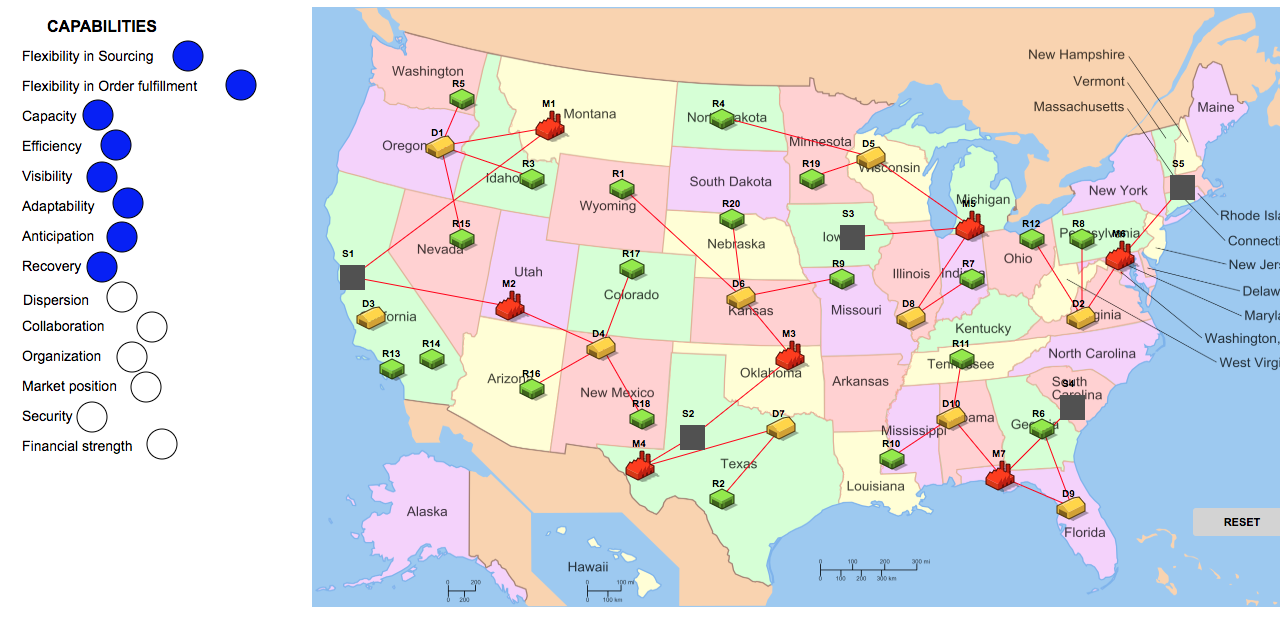
\includegraphics[width=6.5in]{figures/pdf/S3DLD.png}\\
  \caption{Scenario III (Distributor Level Disruption)}
  {The distributor D3 is getting disrupted due to which the retailers associated with it are left unsatisfied. The manufacturer facility M2 is holding the inventory required by the disrupted facility D3. The capabilities associated with this type of disruption are being identified.}
  \label{S3DL}
\end{figure}   

The Fig \ref{S3DL} exhibits the disruption occurring at the distributor facility D3. Due to this disruption, the retailers R13 and R14 along with the manufacturing facility M2 gets disconnected from D3. The retailers R13 and R14 have their demands unfulfilled due to this. There is a need for selecting an alternate source for distributor. This is made possible through the contingency planning component. The alternate distributor is selected in the similar manner as shown in \ref{ALTD}. The key indicator identification reduces the lost time ($T_{\text{L}}$) while the time for recovery ($T_{\text{R}}$) remains the same as that of equation \ref{3.8}. The resiliency of the system is improved by this reduction in time.

\begin{equation}
    Resiliency(R_S) = \frac{6}{18} = 33.33 \% \label{3.23}
\end{equation}

The resiliency and robustness considerations increase the resilience of the supply chain from 16.67 \% to 33.33 \% .

\begin{figure}[H]
  \centering
  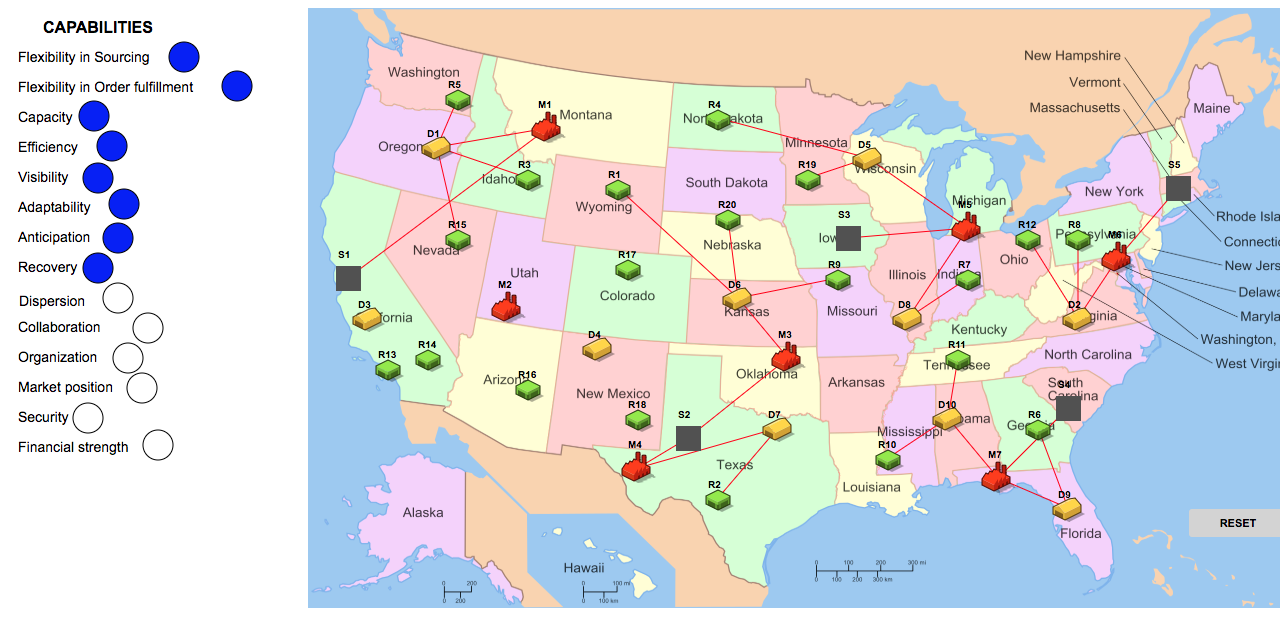
\includegraphics[width=6.5in]{figures/pdf/S3MLD.png}\\
  \caption{Scenario III (Manufacturer Level Disruption)}
  {The manufacturer M2 is getting disrupted due to which the  distributors and retailers associated with it are left unsatisfied. The supplier facility S1 is holding the inventory required by the disrupted facility M2. The capabilities associated with this type of disruption are being identified.}
  \label{S3ML}
\end{figure}   

In the Fig \ref{S3ML} the manufacturing facility M2 is disrupted thus causing the facilities linked with it to disconnect. The demands of the distributors and retailers linked with it are left dissatisfied. These distributors are relocated to a different manufacturer till the recovery of the M2 facility takes place. This relocation is done through the contingency planning component. The reduction in the lost time ($T_{\text{L}}$) through the identification component increases the resilience of the supply chain. The recovery time ($T_{\text{R}}$) is the same as equation \ref{3.9}. 

\begin{equation}
    Resiliency(R_S) = \frac{12}{54} = 22.23 \% \label{3.24}
\end{equation}

The resiliency and robustness considerations increase the resilience of the supply chain from 15.38 \% to 22.23 \% .

\begin{figure}[H]
  \centering
  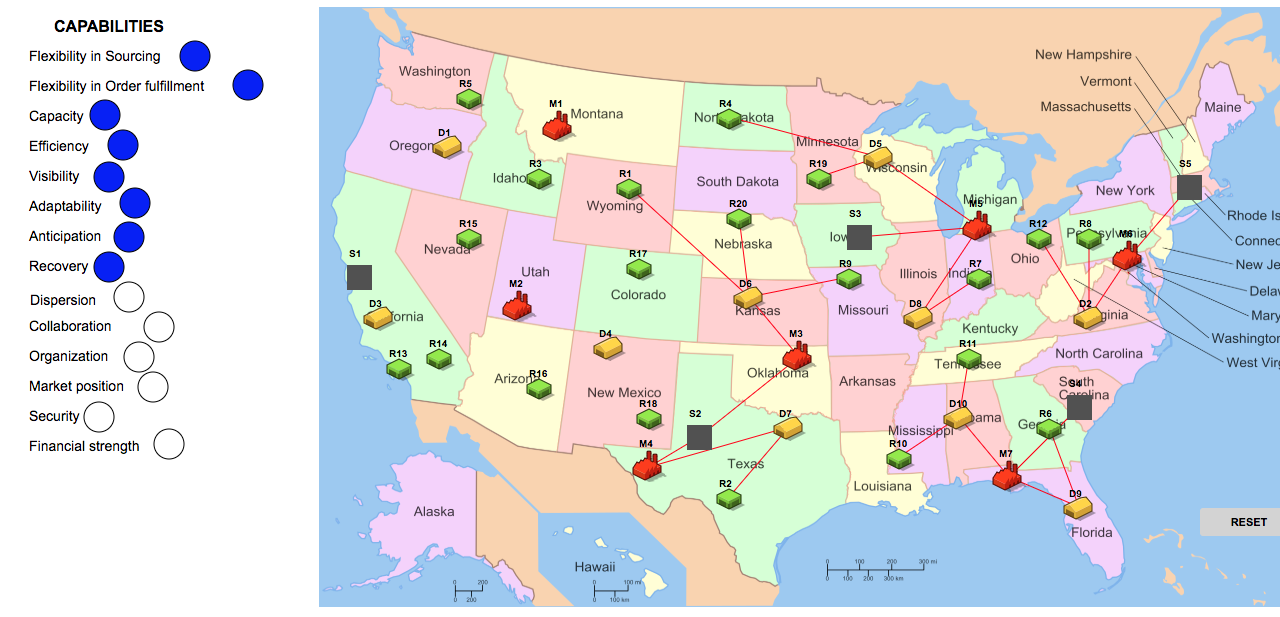
\includegraphics[width=6.5in]{figures/pdf/S3SLD.png}\\
  \caption{Scenario III (Supplier Level Disruption)}
   {The Supplier S1 is getting disrupted due to which the manufactures, distributors, and retailers are left unsatisfied. The entire supply chain is waiting for the facility S1 to be recovered for gaining back the functionality. The capabilities associated with this type of disruption are being identified.}
  \label{S3SL}
\end{figure}   

The Fig \ref{S3SL} depicts the disruption taking place at the supplier facility S1 in the supply chain. The whole supply chain has to wait on its recovery for receiving the materials as it is the sole supplier of the entire supply chain. The contingency planning component allots an alternate supplier facility to the manufacturers M1 and M2 associated with the supplier S1 and maintains a continuous flow of materials in the supply chain. The identification components brings down the lost time ($T_{\text{L}}$) while the recovery time ($T_{\text{R}}$) is the same as that of equation \ref{3.10}. There is an improvement observed in the resiliency of the supply chain because of this.

\begin{equation}
    Resiliency(R_S) = \frac{18}{96} = 18.75 \% \label{3.25}
\end{equation}

The resiliency and robustness considerations increase the resilience of the supply chain from 12.5 \% to 18.75 \%.

\subsubsection{SCENARIO IV: Disruptions due to Connectivity}

In this scenario, the supply chain face disruptions due to uncertainties in the connectivity. These arise from any complications in the scale of network, reliance upon information, and degree of outsourcing. The key indicators linked to this type of disruptions are the capabilities of visibility, adaptability, recovery, and security. The facilities at all the levels of disruption are kept the same. 

\subsubsection{Distributor Level disruption}

\begin{figure}[H]
  \centering
  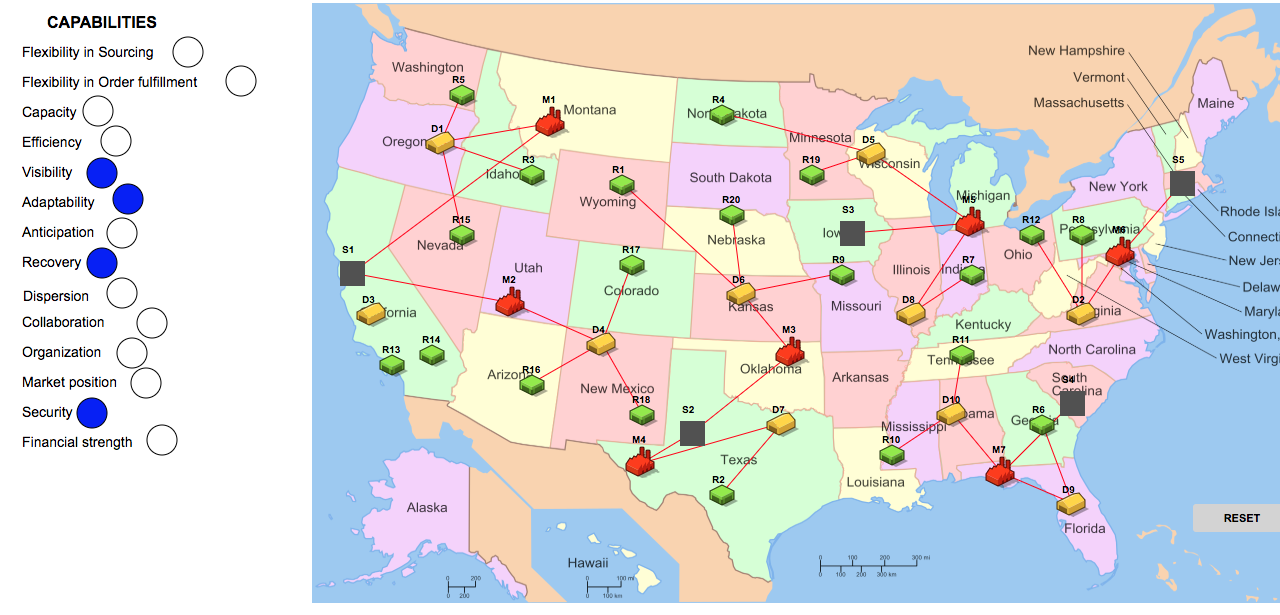
\includegraphics[width=6.5in]{figures/pdf/S4DLD.png}\\
  \caption{Scenario IV (Distributor Level Disruption)}
  {The distributor D3 is getting disrupted due to which the retailers associated with it are left unsatisfied. The manufacturer facility M2 is holding the inventory required by the disrupted facility D3. The capabilities associated with this type of disruption are being identified.}
  \label{S4DL}
\end{figure}   

The Fig \ref{S4DL} shows the distributed facility D3 and the effects it has on its linked facilities. The retailers R13 and R14 have to move to a different distributor for getting their demands satisfied. The contingency planning selects an alternate distributor facility for these retailers in the similar manner as shown in Fig \ref{ALTD}. The lost time ($T_{\text{L}}$) is reduced to 18 hours while the recovery time ($T_{\text{R}}$) remains the same as that of equation \ref{3.11}. The resiliency of the supply chain is then calculated as 

\begin{equation}
    Resiliency(R_S) = \frac{11}{18} = 61.11 \% \label{3.26}
\end{equation}

The resiliency and robustness considerations increase the resilience of the supply chain from 30.56 \% to 61.11 \%.

\begin{figure}[H]
  \centering
  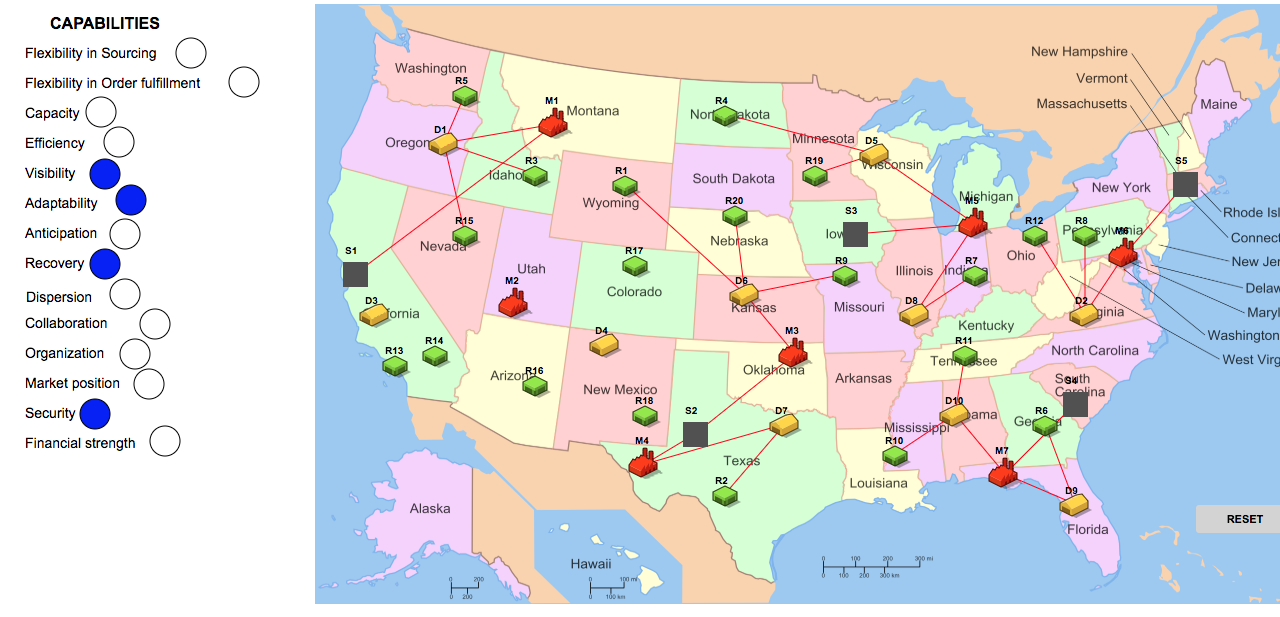
\includegraphics[width=6.5in]{figures/pdf/S4MLD.png}\\
  \caption{Scenario IV (Manufacturer Level Disruption)}
  {The manufacturer M2 is getting disrupted due to which the  distributors and retailers associated with it are left unsatisfied. The supplier facility S1 is holding the inventory required by the disrupted facility M2. The capabilities associated with this type of disruption are being identified.}
  \label{S4ML}
\end{figure}   

The disrupted manufacturer M2 is shown in Fig \ref{S4ML} along with the key indicators identification. This leads to the disconnection of D3 and D4 facilities to get disconnected from M2. Thus, the retailers associated with these distributors get affected. The alternate manufacturer is selected for these distributors with the help of contingency planning in the same way as shown in Fig \ref{ALTM} till the M2 facility recovers. The resiliency is increased by the incursion of key capabilities identification. The lost time ($T_{\text{L}}$) is reduced to 17 hours while the recovery time ($T_{\text{R}}$) remains the same as that of equation \ref{3.12}. 

\begin{equation}
    Resiliency(R_S) = \frac{17}{54} = 31.48 \% \label{3.27}
\end{equation}

The resiliency and robustness considerations increase the resilience of the supply chain from 21.79 \% to 31.48 \%.

\begin{figure}[H]
  \centering
  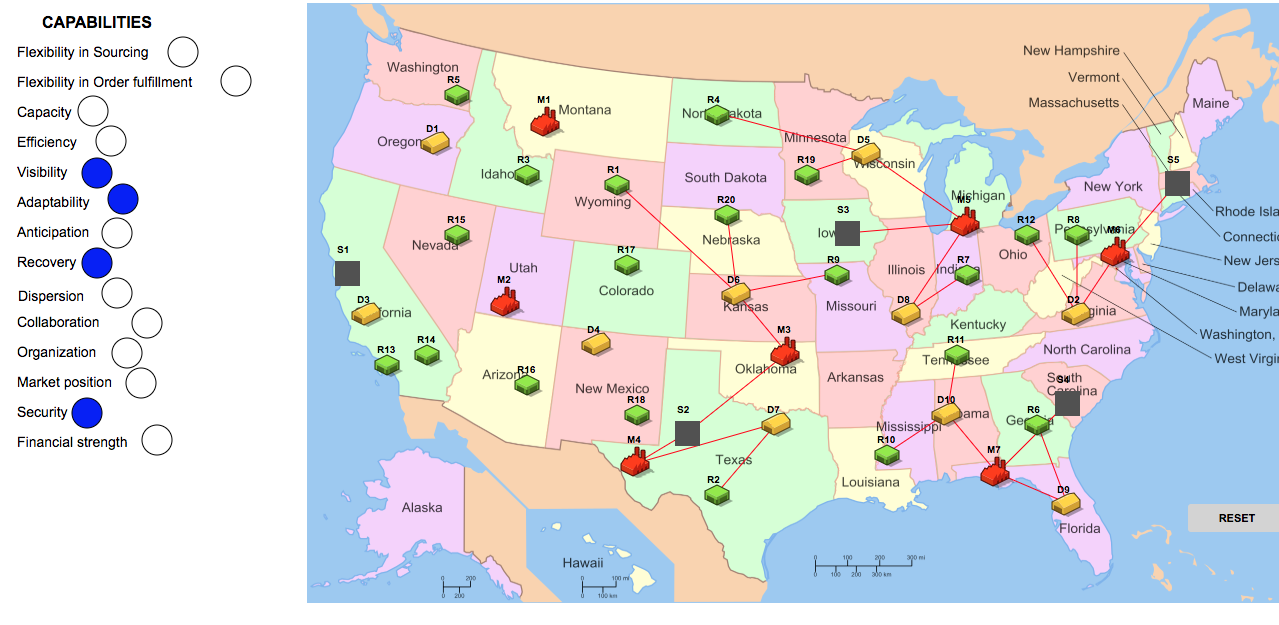
\includegraphics[width=6.5in]{figures/pdf/S4SLD.png}\\
  \caption{Scenario IV (Supplier Level Disruption)}
  {The Supplier S1 is getting disrupted due to which the manufactures, distributors, and retailers are left unsatisfied. The entire supply chain is waiting for the facility S1 to be recovered for gaining back the functionality. The capabilities associated with this type of disruption are being identified.}
  \label{S4SL}
\end{figure}  

The Fig \ref{S4SL} shows the supplier S1 being disrupted and the key indicators being identified. The contingency planning allocates a new supplier for the manufacturing facilities M1 and M2 which are completely reliant on the S1 facility. The new supplier is selected for M1 and M2 in the same way as shown in Fig \ref{ALTS}. The lost time ($T_{\text{L}}$) is reduced to 23 hours due to the identification component while the recovery time ($T_{\text{R}}$) remains the same as that of equation \ref{3.13}.

\begin{equation}
    Resiliency(R_S) = \frac{23}{96} = 23.95 \% \label{3.28}
\end{equation}

The resiliency and robustness considerations increase the resilience of the supply chain from 15.79 \% to 23.95 \%.

\subsubsection{SCENARIO V: Disruptions due to Deliberate Threats}

In this scenario, the disruption in the supply chain is caused due to the deliberate threats. These disruptions occur mainly due to labor disputes, theft, and terrorism/sabotage. The key capabilities associated with this type of disruption are identified as security, anticipation, and collaboration. The facilities which get affected are the same at all levels of disruptions in the supply chain.

\subsubsection{Distributor Level Disruption}

\begin{figure}[H]
  \centering
  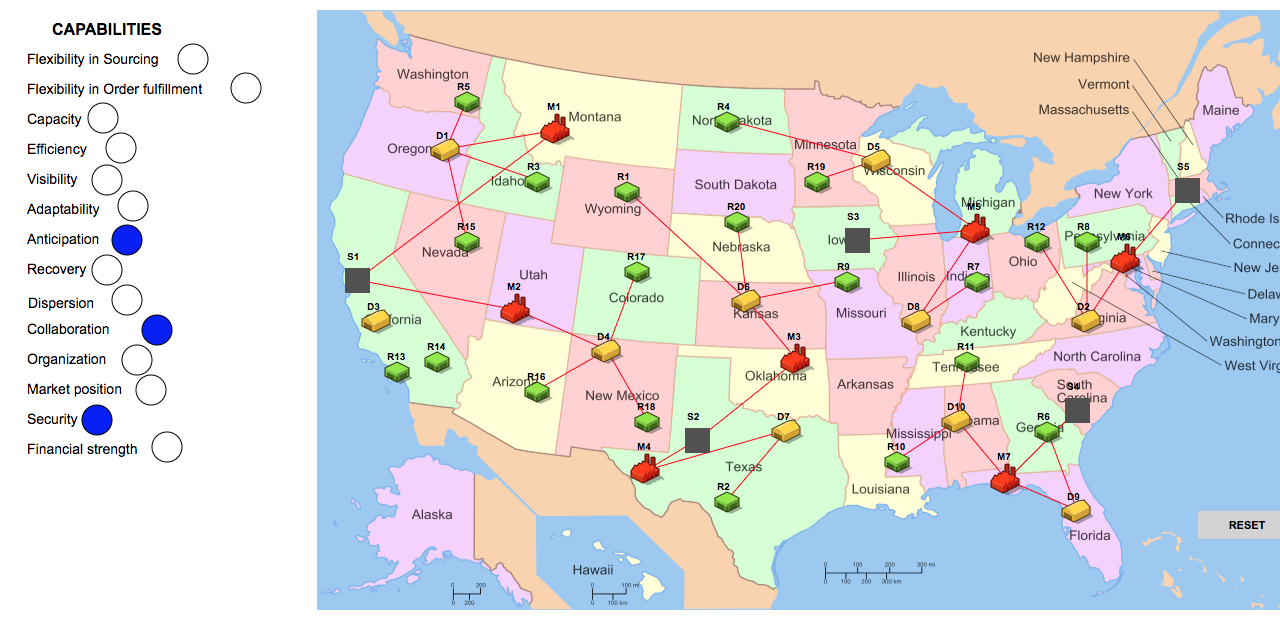
\includegraphics[width=6.5in]{figures/pdf/S5DLD.png}\\
  \caption{Scenario V (Distributor Level Disruption)}
  {The distributor D3 is getting disrupted due to which the retailers associated with it are left unsatisfied. The manufacturer facility M2 is holding the inventory required by the disrupted facility D3. The capabilities associated with this type of disruption are being identified.}
  \label{S5DL}
\end{figure}   
 
The Fig \ref{S5DL} displays the distributor facility D3 being disrupted and the key indicators being identified. The retailers R13 and R14 along with the manufacturer M2 get disconnected from the D3 facility. The contingency planning component allocates a different distributor facility in the same way as shown in Fig \ref{ALTD} while the disrupted D3 facility is recovered. The lost time ($T_{\text{L}}$) is reduced to 18 hours while the recovery time ($T_{\text{R}}$) is the same as that of equation \ref{3.14}. The resiliency of the supply chain is thus found out as

\begin{equation}
    Resiliency(R_S) = \frac{10}{18} = 55.55 \% \label{3.29}
\end{equation}

The resiliency and robustness considerations increase the resilience of the supply chain from 27.78 \% to 55.55 \%.

\begin{figure}[H]
  \centering
  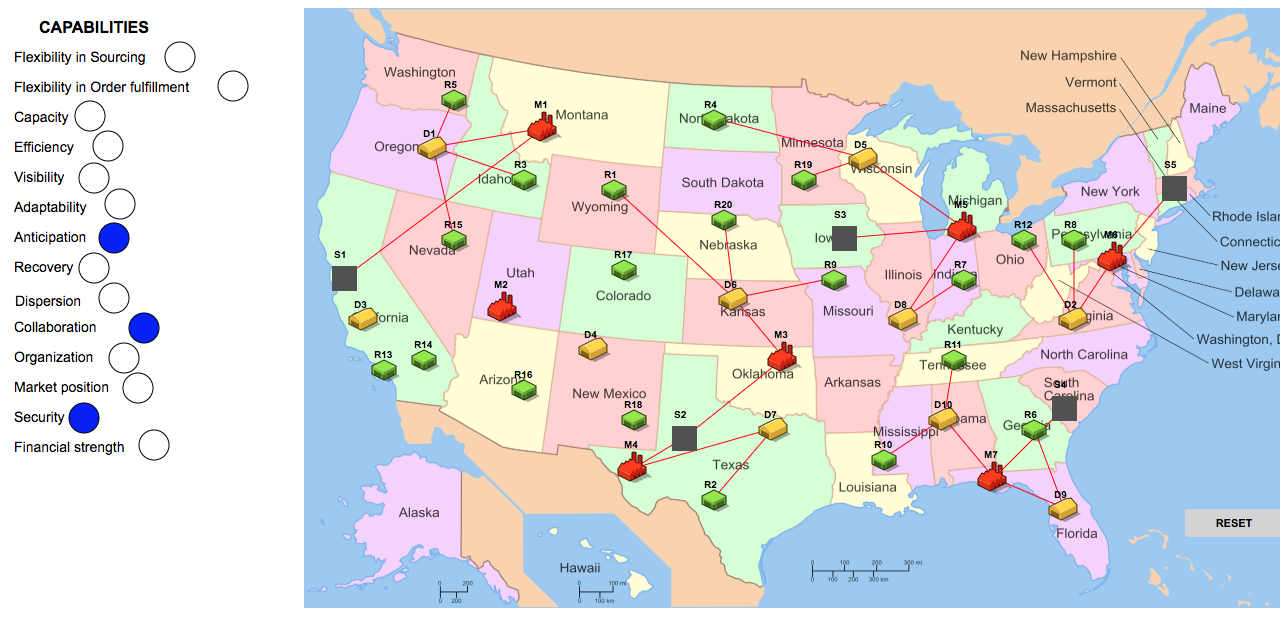
\includegraphics[width=6.5in]{figures/pdf/S5MLD.png}\\
  \caption{Scenario V (Manufacturer Level Disruption)}
  {The manufacturer M2 is getting disrupted due to which the  distributors and retailers associated with it are left unsatisfied. The supplier facility S1 is holding the inventory required by the disrupted facility M2. The capabilities associated with this type of disruption are being identified.}
  \label{S5ML}
\end{figure}   

The manufacturing facility M2 is disrupted and the key capabilities are indicated as shown in the Fig \ref{S5ML}. The contingency planning selects an alternate manufacturing facility for the distributors D3 and D4 which are associated with the disrupted facility M2. This is selection is done similar to that as shown in the Fig \ref{ALTM} while the disrupted facility recovers. The identification element decreases the lost time ($T_{\text{L}}$) to 16 hours while the recovery time ($T_{\text{R}}$) remains the same as that of equation \ref{3.15}. The resiliency value of the supply chain is calculated as

\begin{equation}
    Resiliency(R_S) = \frac{16}{54} = 29.62 \% \label{3.30}
\end{equation}

The resiliency and robustness considerations increase the resilience of the supply chain from 20.54 \% to 29.62 \%.

\begin{figure}[H]
  \centering
  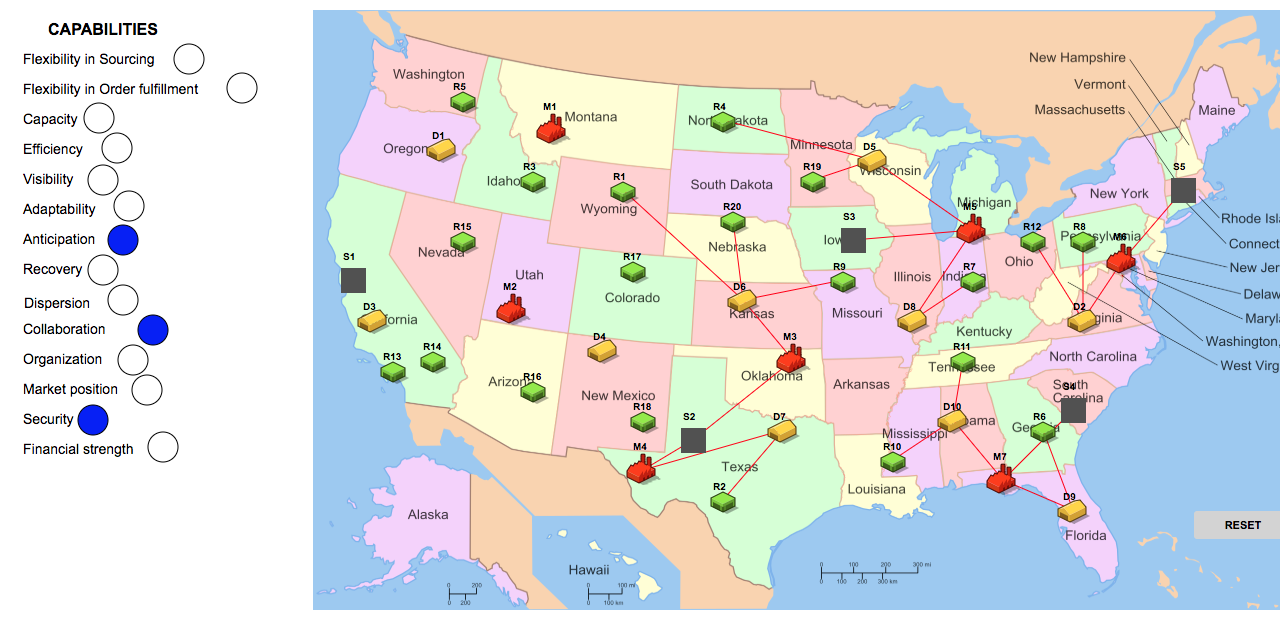
\includegraphics[width=6.5in]{figures/pdf/S5SLD.png}\\
  \caption{Scenario V (Supplier Level Disruption)}.
  {The Supplier S1 is getting disrupted due to which the manufactures, distributors, and retailers are left unsatisfied. The entire supply chain is waiting for the facility S1 to be recovered for gaining back the functionality. The capabilities associated with this type of disruption are being identified.}\label{S5SL}
\end{figure}  

In the Fig \ref{S5SL} the disrupted supplier facility S1 is displayed along with the key indicators being identified at the time of the disruption. Alternate supplier facility for the manufacturers M1 and M2 is done through contingency planning so that the continuous supply chain is achieved. This supplier is selected the same way as shown in the Fig \ref{ALTS}. The resiliency is improved by the application of the identification element in the supply chain. The lost time ($T_{\text{L}}$) is lowered to 22 hours while the recovery time ($T_{\text{R}}$) remains the same as that of equation \ref{3.16}. The supply chain resiliency is then given as

\begin{equation}
    Resiliency(R_S) = \frac{22}{96} = 22.91 \% \label{3.31}
\end{equation}

The resiliency and robustness considerations increase the resilience of the supply chain from 15.27 \% to 22.91 \%.

The resiliency values for all the scenarios at all the levels right from the equation \ref{3.2} to equation \ref{3.31} are accrued together and are put in a tabular form and are shown in the Fig \ref{RESV} for observing the improvements in the supply chain resiliency before and after the consideration of resiliency and robustness

\begin{figure}[H]
  \centering
  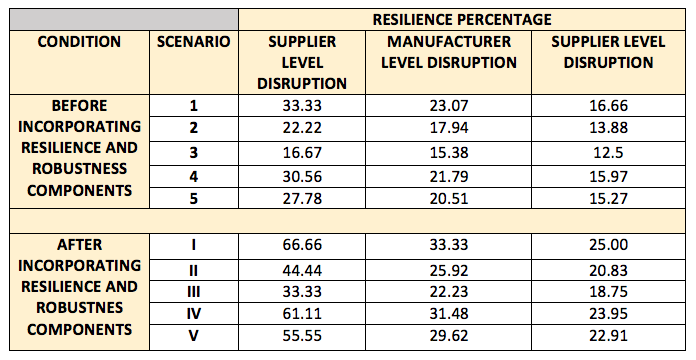
\includegraphics[width=6.5in]{figures/pdf/ResilienceValues.png}\\
  \caption{All the Resilience values}\label{RESV}
\end{figure}  



\begin{figure}[H]
  \centering
  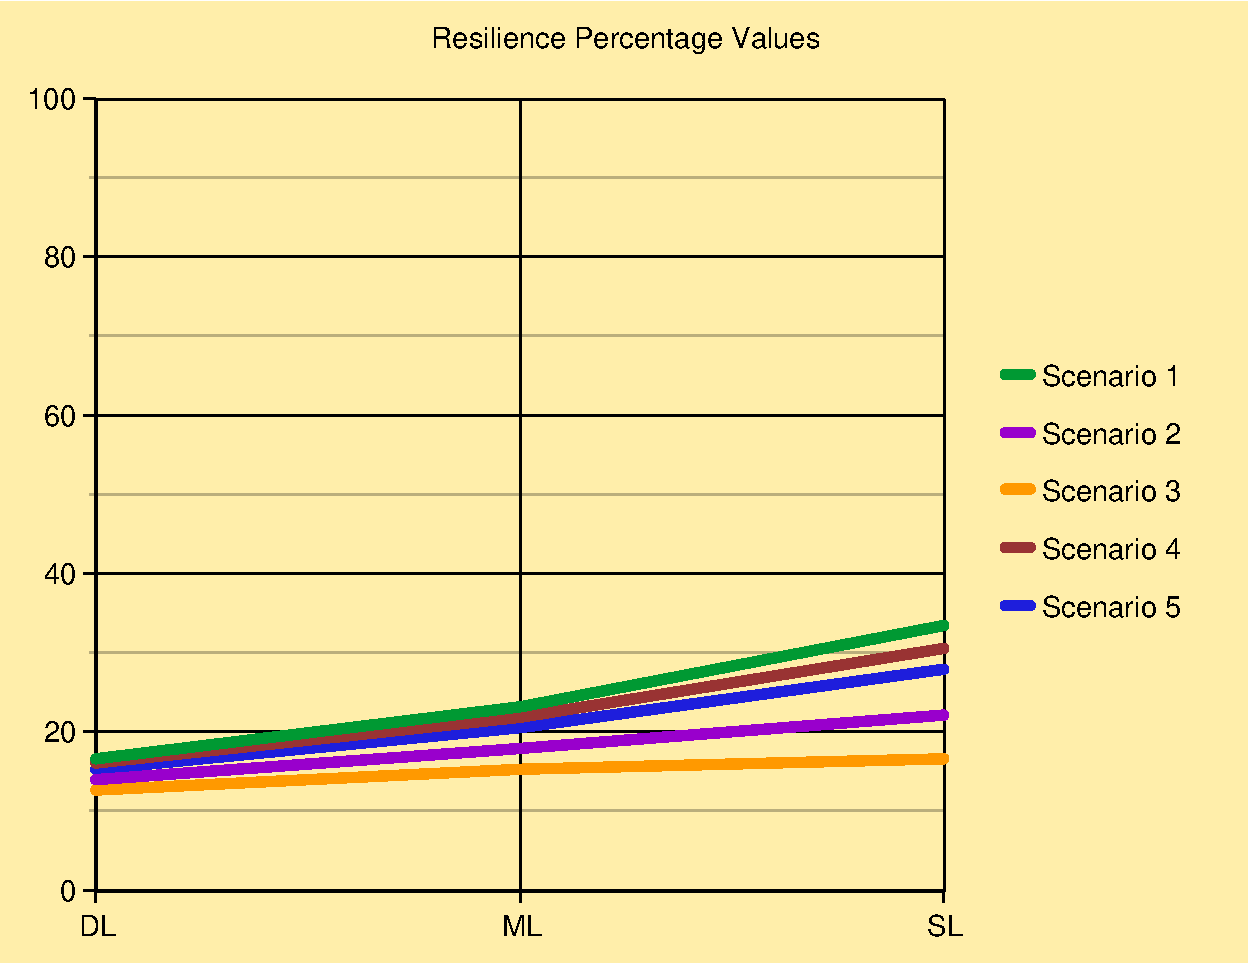
\includegraphics[width=5.5in]{figures/pdf/Before(Graph).pdf}\\
  \caption{Graph for the Resiliency values for the Supply Chain before incorporating Resilience and Robustness Components}\label{G1}
\end{figure}  

It is clearly evident that there is an improvement in all the scenarios after the inclusion on resilience and robustness components in the design of the supply chain. These values when plotted on a graph describe the difference between the two strategies very efficiently. The Fig \ref{G1}shows the graph of the values of all the values of the resiliency obtained before including the resiliency and robustness components. After these components are included in the supply chain, the resilience percentage values increase for the disruptions occurring at all the levels. This can be seen from the graph in Fig \ref{G2}.

\begin{figure}[H]
  \centering
  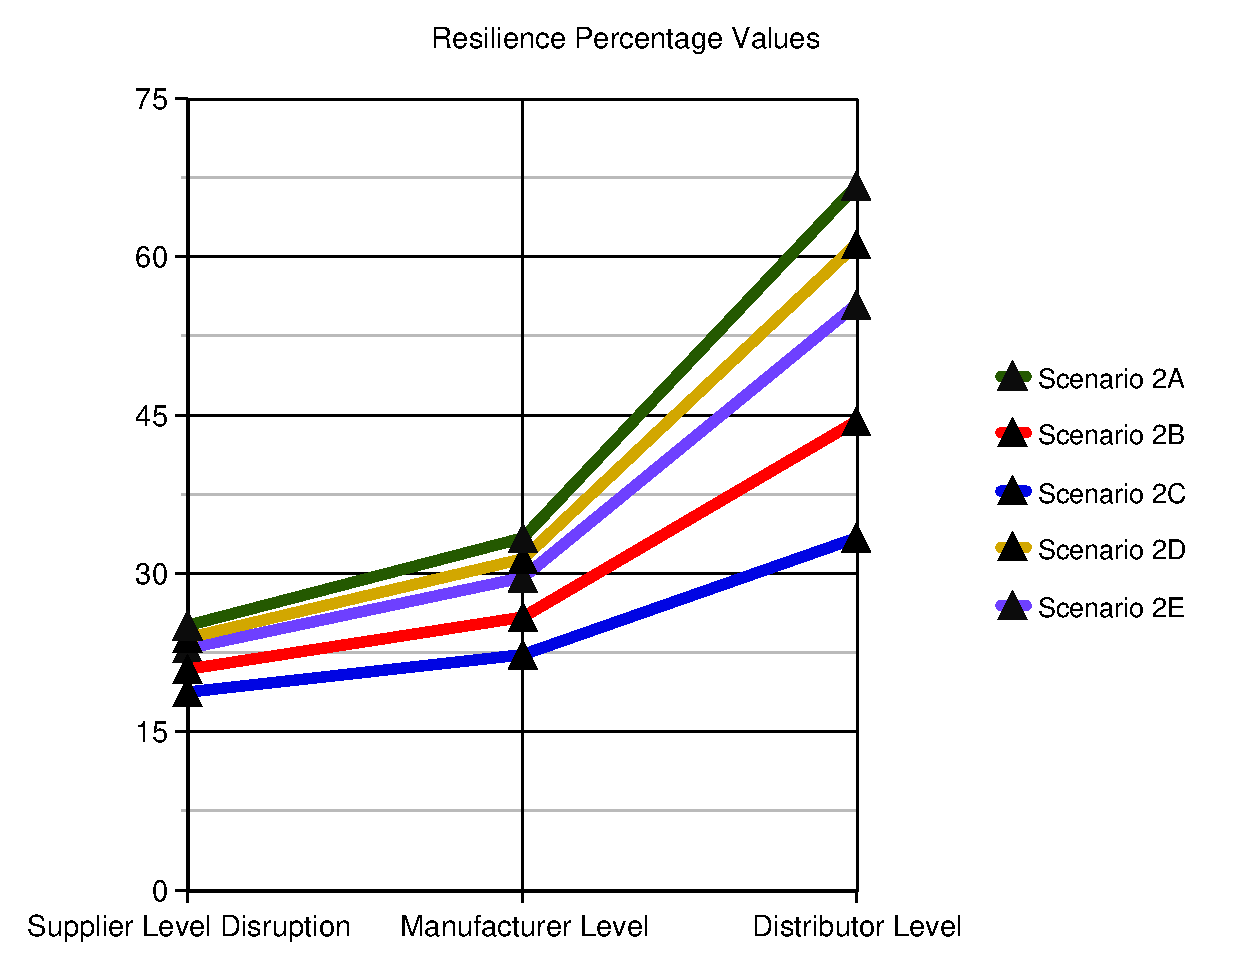
\includegraphics[width=5.5in]{figures/pdf/After(Graph).pdf}\\
  \caption{Graph for the Resiliency values for the Supply Chain after incorporating Resilience and Robustness Components}\label{G2}
\end{figure}  
    \chapter{Case Study} \label{ch:casestudy}

In the supply chain model as mentioned in the methodology section, we are considering the supply chain consisting of 5 Suppliers, 7 Manufacturers, 10 Distributors, and 20 Retailers as our case study. This supply chain model is then subjected to different sources of disruption. The results of the resilience value for modeling with and without the resiliency and robustness enhancers are compared for quantifying the methodology. This case study can be considered for generic design purposes as well. The values of the parameters for the Suppliers are as shown in the Table \ref{tab:Supplier}. The parameters for the manufacturer agent and their corresponding values are shown in the Table \ref{tab:Manufacturer}. The parameters for the distributor agent and the values associated with them are as shown in the Table \ref{tab:Distributor}. The values corresponding to this parameter for the retailer agent is as shown in the Table \ref{tab:Retailer}. The costs such as inventory holding cost and backlog cost together make the total cost (lost) in the supply chain. Theses costs are used for the quantification of our methodology.


\begin{table}[H]
\caption{Parameters of the Supplier}
\label{tab:Supplier}
\begin{center}
\begin{tabular}[b]{|c|c|c|}
	\hline
	Supplier & Raw Material Handling Cost & Response Time \\ \hline
	S1 & 0.45 & High\\ \hline
	S2 & 0.52 & Medium \\ \hline
	S3 & 0.44 & High \\ \hline
	S4 & 0.58 & Low \\ \hline
	S5 & 0.56 & Medium \\ \hline
\end{tabular}
\end{center}
\end{table}

\begin{table}[H]
\caption{Parameters of the Manufacturer}
\label{tab:Manufacturer}
\begin{center}
\begin{tabular}[b]{|c|c|c|}
	\hline
	Manufacturer & Inventory Holding Cost & Response Time \\ \hline
	M1 & 0.51 & Low\\ \hline
	M2 & 0.41 & Medium \\ \hline
	M3 & 0.43 & Medium \\ \hline
	M4 & 0.57 & High \\ \hline
	M5 & 0.49 & Low \\ \hline
	M6 & 0.55 & High \\ \hline
	M7 & 0.48 & Low \\ \hline
\end{tabular}
\end{center}
\end{table}

\begin{table}[H]
\caption{Parameters of the Distributor}
\label{tab:Distributor}
\begin{center}
\begin{tabular}[b]{|c|c|c|c|}
	\hline
	Distributor & Inventory Holding Cost & Order Fulfillment Rate & Response Time \\ \hline
	D1 & 0.46 & High & Medium\\ \hline
	D2 & 0.51 & High & High \\ \hline
	D3 & 0.44 & Low & Low \\ \hline
	D4 & 0.52 & High & High \\ \hline
	D5 & 0.48 & Low & Medium \\ \hline
	D6 & 0.49 & Low & Low \\ \hline
	D7 & 0.57 & High & Low \\ \hline
    D8 & 0.41 & High & Medium \\ \hline
    D9 & 0.48 & High & High \\ \hline
    D10 & 0.53 & Low & Low \\ \hline
\end{tabular}
\end{center}
\end{table}

\begin{table}[H]
\caption{Parameters of the Retailer}
\label{tab:Retailer}
\begin{center}
\begin{tabular}[b]{|c|c|}
	\hline
	Retailer & Response Time \\ \hline
	R1 & Low \\ \hline
	R2 & Medium \\ \hline
	R3 & Low \\ \hline
	R4 & High \\ \hline
	R5 & High \\ \hline
	R6 & Medium \\ \hline
	R7 & High \\ \hline
	R8 & Low \\ \hline
	R9 & Low \\ \hline
	R10 & Medium \\ \hline
	R11 & High \\ \hline
	R12 & Low \\ \hline
	R13 & Medium \\ \hline
	R14 & Medium \\ \hline
	R15 & High \\ \hline
	R16 & High \\ \hline
	R17 & High \\ \hline
	R18 & Low \\ \hline
	R19 & High \\ \hline
	R20 & Medium \\ \hline
\end{tabular}
\end{center}
\end{table}

\newpage
\section{The Base Model Connections}
The four agent types are connected to each other to form 5 supply chains in the different regions throughout the country for a company. In the base model, the connections of the agents is as shown in the Fig \ref{Base}. It can be observed from the Fig \ref{Base} that the distributor D1 is shared by three retailers R3, R5 and R15. If there is a disruption in the area of Oregon and the distributor D1 is down due to it, then the retailers R3, R5, and R15 have to select a different distributor facility. They will choose the distributors from D2 to D10 based on who has the best parameter values. Similarly, the distributor agents and manufacturer agents connect to the best available manufacturer agent and supplier agent respectively based on the parameters. In the meantime, the restoration of the disrupted facility is taking place using appropriate mitigation strategies. This is the basic working logic of the whole simulation model. The run time of the simulation for our model is 365 days and the three different scenarios are at distributor level, at manufacturer level, and at supplier level. Theses three scenarios are considered under normal working conditions, under disruption conditions, and under disruption conditions with contingency planning. Out of these three scenarios, we have considered the scenario for disruptions at the manufacturer level.

\begin{figure}[H]
  \centering
  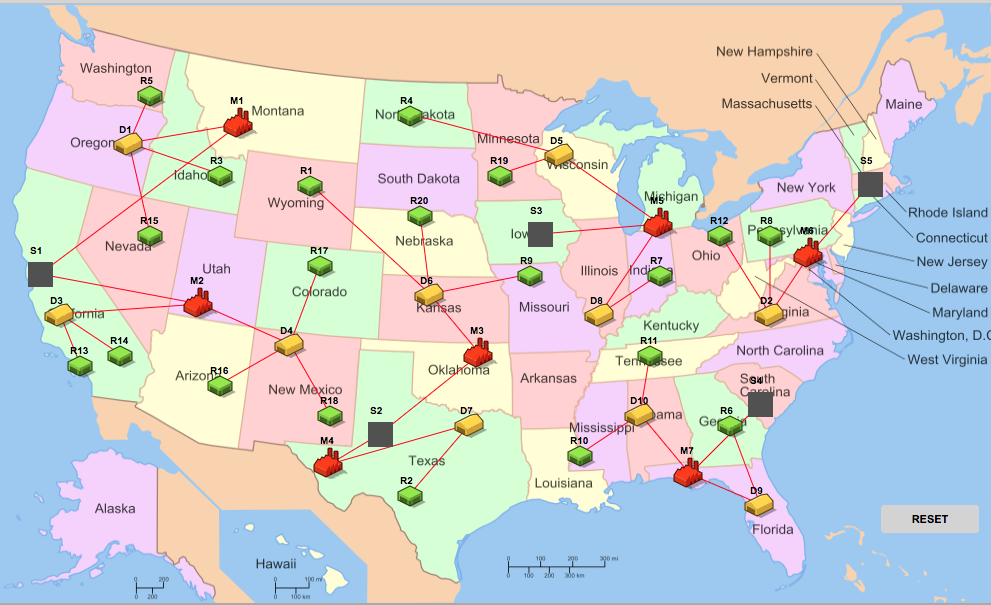
\includegraphics[width=4.0in]{figures/pdf/Basic-connections.png}\\
  \caption{Base Model Agent Connections.}\label{Base}
\end{figure}


\section{Modeling for disruptions at the Manufacturer Level}
 In this model, the connections of the supply chain are as shown in the Fig \ref{Base}. There are three scenarios that can be observed for the behavior of supply chain at the manufacturer level. These scenarios are the supply chain under normal conditions, the supply chain under disruption condition, and the supply chain under disruption condition with contingency planning. The various sources of disruption are considered for these three scenarios. The total costs (lost) and the resiliency values corresponding to these scenarios are calculated.  
 
 \subsection{Supply Chain Performance under Normal Conditions}
In this scenario, the supply chain at manufacturer level is functioning under normal conditions. There exists losses in terms of cost due to the uncertainty of demands and unavailability of the inventory at certain facilities. These losses are due to the inventory holding costs and the backlog costs. The total costs incurred at the three different zones as shown in fig \ref{Base} are \$39,973.4, \$63,139.25, and \$15,842.02 for zones 1, 2, and 3 respectively. The next step is to find out these values under the conditions of disruption. The manufacturing facilities in the three different zones are disrupted at random and the performance of the supply chain is monitored.

 \subsection{Supply Chain Performance under Disruption Conditions}

In this scenario, we have disrupted the different manufacturers which are located in the entire supply chain across the entire geographical United States of America. As these manufacturers are down, the effects of disruption spread throughout the supply chain through the facilities linked with them. This occurs due to the phenomenon known as ripple effect. As the manufacturers supply for the distributors, the distributors are unable to collect the finished goods and fulfill the demand for the retailers associated with them. As a result, the retailers are unable to fulfill the demands of the customers in their region. Thus, a backlog takes place both at the retailers and distributors. The suppliers linked to the manufacturers have to hold the excess raw materials at their facility due to the uncertain duration of recovery of the disrupted facility. The connections before and after the disruption at one such manufacturer facility M2 are shown in the Fig \ref{fig:MLDb} and Fig \ref{fig:MLDa}. The disruption causes the facilities R13, R14, R16, R17, R18, D3, and D4 to become inactive. The supplier S1 gets disconnected from the manufacturer M2.

The lost time and recovery time occurred during different scenarios has a different value. Apart from the loss of time, there are other ramifications such as the backlog cost, inventory holding cost and the loss of customer loyalty. The disruptions take place at the manufacturer level over the period of 365 days. In this period, there are 18 different disruptions which are caused due to the different sources of disruption which are mentioned in the methodology section. This causes a delay of 126 days in the supply chain. Out of these 126 days, the repair time ($T_{\text{N}}$) comprises of 54 days. The lost time ($T_{\text{L}}$) in this scenario is of 72 days. Thus, the recovery time of this scenario is calculated as follows.

\begin{equation}
    T_R = T_N + T_L = 54 + 72 = 126  \label{3.3}
\end{equation}

The total cycle time ($T_{\text{C}}$) in this scenario is of 239 days. The total time of the system now becomes the sum of the total cycle time ($T_{\text{C}}$) and the recovery time ($T_{\text{R}}$). Thus, the resilience value for this scenario is calculated as follows.

\begin{equation}
  R_S = \frac{T}{T_R} = \frac{365}{126} = 2.89  \label{existing}
\end{equation}

The resilience value from the equation \ref{existing} is the existing resilience value ($R_{\text{existing}}$) of the supply chain. The total costs suffered due to the disruptions which comprise of the inventory holding cost and the backlog costs for zones 1, 2, and 3 are \$159,090.8, \$145,987.25, and \$184,948.28 respectively. These heavy losses are suffered due to the absence of mitigation and resilient strategies in the design of the supply chain.

 \begin{figure}[H]
   \centering
    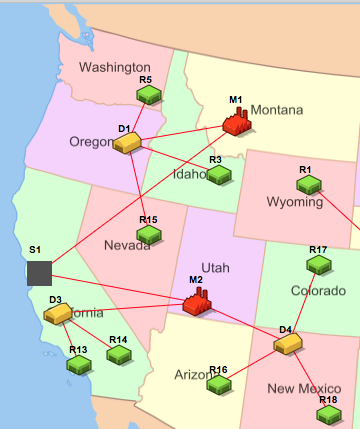
\includegraphics[width=3.0in]{figures/pdf/BeforeM.png} 
    \caption{Manufacturer Level Disruption (Before).}
    \label{fig:MLDb}
\end{figure}

\begin{figure}[H]
    \centering
   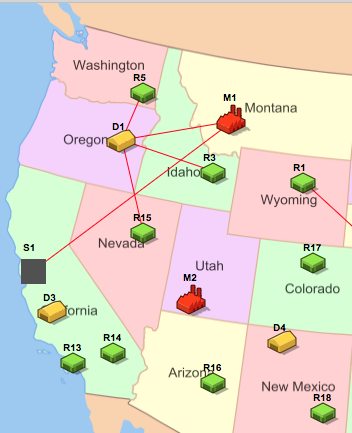
\includegraphics[width=3.0in]{figures/pdf/AfterM.png}
   \caption{Manufacturer Level Disruption (After).}
   \label{fig:MLDa}
\end{figure}

\subsection{Supply Chain Performance under Disruption Conditions with Contingency Planning and Key Indicators Identification}
In this scenario, we have implemented the key indicator identification and contingency planning components into our supply chain. Whenever a disruption takes place, the source of the disruption is identified and a team of management personnel look into the capabilities that need to be strengthened in order to reduce the recovery time. In the meantime, an alternate facility having the least distance, lowest costs, high fulfillment rate, and low response time is selected from the other available facilities. There is transportation cost that is incurred due to alternate facility location. But, this cost is just a small price to pay in order to avoid huge losses if we wait for the damaged facility to be repaired. The lost time is reduced by a drastic amount and thus the total delay caused by the disruption is reduced while keeping the supply chain working simultaneously. Thus, a resilient and robust supply chain is achieved.

In this period, there are 18 different disruptions which are caused due to the different sources of disruption which are mentioned in the methodology section. In this scenario due to the inclusion of resilience techniques such as contingency planning and key indicators identification, there is a delay of 72 days in the supply chain. Out of these 72 days, the repair time ($T_{\text{N}}$) comprises of 54 days. The lost time ($T_{\text{L}}$) in this scenario is of 18 days. Thus, the recovery time of this scenario is calculated as follows.

\begin{equation}
    T_R = T_N + T_L = 54 + 18 = 72  \label{3.3}
\end{equation}

 The total time of the system now becomes the sum of the total cycle time ($T_{\text{C}}$) and the recovery time ($T_{\text{R}}$) which is 365 days. Thus, the resilience value for this scenario is calculated as follows.

\begin{equation}
  R_S = \frac{T}{T_R} = \frac{365}{72} = 5.0694  \label{new}
\end{equation}

The resilience value from the equation \ref{new} is the existing resilience value ($R_{\text{new}}$) of the supply chain. The percentage change in the resilience value can now be calculated as follows.

\begin{equation}
      \% change in resilience = \frac{5.0694 - 2.89}{2.89} * 100 = 75.411 \%  \label{res}
\end{equation}

The equation \ref{res} represents the improvement achieved in the resilience value after incorporating the resilience factors in the supply chain. The total costs suffered due to the disruptions which comprise of the inventory holding cost and the backlog costs for zones 1, 2, and 3 are \$63,606.4, \$82,938.00, and \$43,773.04 respectively. 

Due to the contingency planning, whenever a manufacturing facility is down due to disruption, an alternate manufacturing facility is provided without much loss in time. This enables for the demand of the distributor facilities associated with the disrupted facility to be satisfied so that the demand of the retailers associated with the distributors can be satisfied. If there is a disruption at the manufacturers in the zone 1, then the distribution facilities D1, D3, and D4 get affected as well. Thus, affecting the retailers R3, R5, R13, R14, R15, R16, R17 and R18. Through contingency planning, in times of disruption, the distribution facilities are allocated the manufacturing facility M4 for the fulfillment of their demands such that the supply chain does not come to a halt. The effect of disruption on the manufacturing facilities in the zone 1 is shown in the fig \ref{Z1BD}. The pictorial representation of the contingency planning for zone 1 is shown in the fig \ref{Z1AD}. Similarly, the effects of disruption on the manufacturing facilities of zone 2 and zone 3 can be seen in the figures \ref{Z2BD} and \ref{Z3BD}. The contingency planning for zone 2 and 3 are shown in figures \ref{Z2AD} and \ref{Z3AD}. Through the key indicators identification, the capabilities associated with the source of the disruption can be utilized for mitigating the effects of the disruption. The capabilities are highlighted in the simulation depending on the duration of the disruptions which identifies the source of disruption. This identification of the capabilities in the simulation software is as shown in figure \ref{V1}, \ref{V2}, \ref{V3}, \ref{V4}, and \ref{V5} for the disruption sources (vulnerabilities) as Turbulence, Supplier/Customer disruptions, Resource Limits, Connectivity, and Deliberate threats. This aids in reducing the recovery time of the supply chain from disruption and reducing the losses incurred.

\begin{figure}[H]
  \centering
  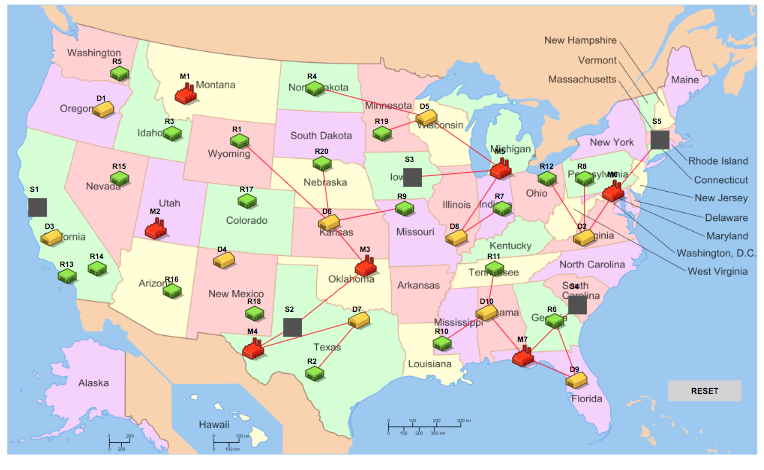
\includegraphics[width=6.5in]{figures/pdf/Z1BD.png}\\
  \caption{Zone 1 during disruption}\label{Z1BD}
\end{figure}  

\begin{figure}[H]
  \centering
  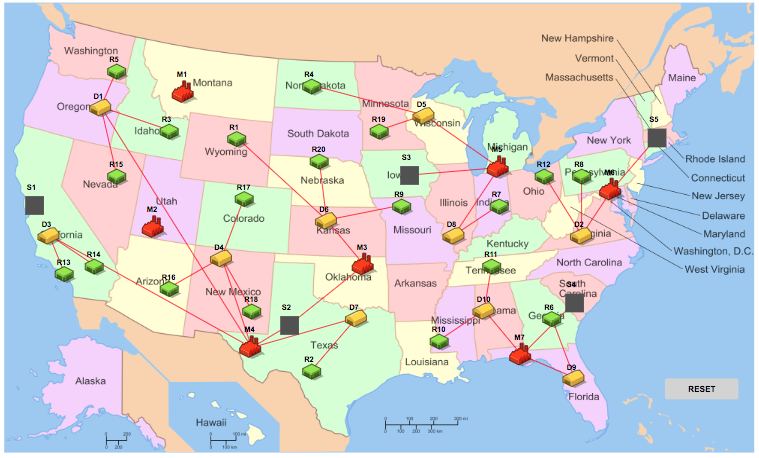
\includegraphics[width=6.5in]{figures/pdf/Z1AD.png}\\
  \caption{Zone 1 after disruption with contingency planning}\label{Z1AD}
\end{figure}  

\begin{figure}[H]
  \centering
  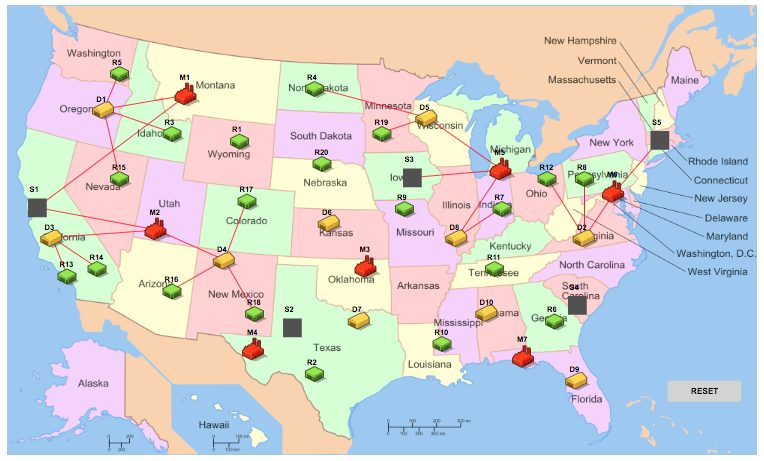
\includegraphics[width=6.5in]{figures/pdf/Z2BD.png}\\
  \caption{Zone 2 during disruption}\label{Z2BD}
\end{figure}  

\begin{figure}[H]
  \centering
  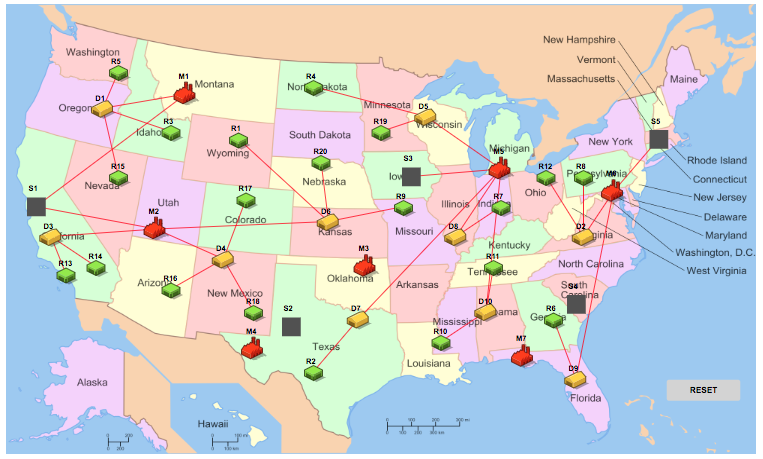
\includegraphics[width=6.5in]{figures/pdf/Z2AD.png}\\
  \caption{Zone 2 after disruption with contingency planning}\label{Z2AD}
\end{figure}  

\begin{figure}[H]
  \centering
  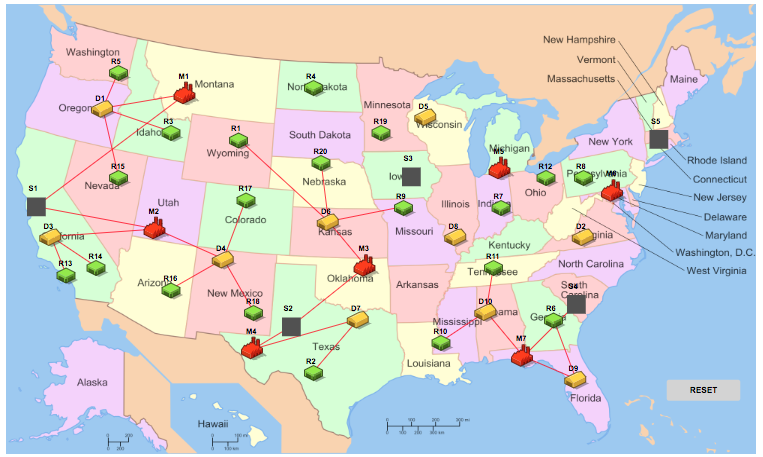
\includegraphics[width=6.5in]{figures/pdf/Z3BD.png}\\
  \caption{Zone 3 during disruption}\label{Z3BD}
\end{figure}  

\begin{figure}[H]
  \centering
  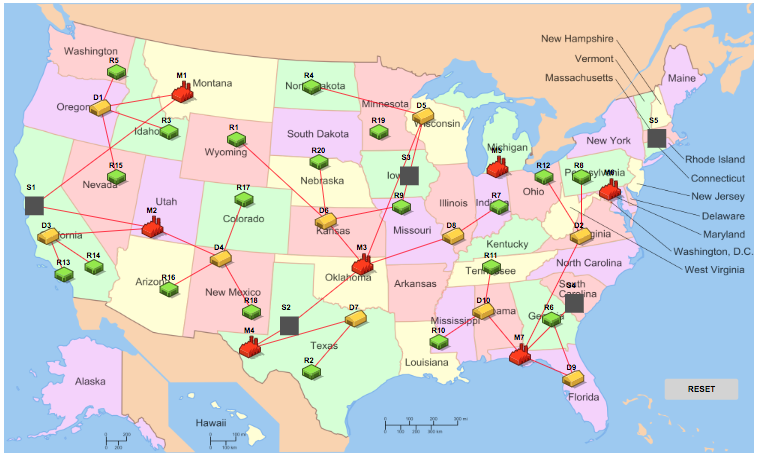
\includegraphics[width=6.5in]{figures/pdf/Z3AD.png}\\
  \caption{Zone 3 after disruption with contingency planning}\label{Z3AD}
\end{figure}  

\begin{figure}[H]
  \centering
  \includegraphics[width=4.5in]{figures/V1.png}\\
  \caption{Capabilities for Vulnerabilities due to Turbulence}\label{V1}
\end{figure}  

\begin{figure}[H]
  \centering
  \includegraphics[width=4.5in]{figures/V2.png}\\
  \caption{Capabilities for Vulnerabilities due to Supplier/Customer disruptions}\label{V2}
\end{figure}  

\begin{figure}[H]
  \centering
  \includegraphics[width=4.5in]{figures/V3.png}\\
  \caption{Capabilities for Vulnerabilities due to Resource Limits}\label{V3}
\end{figure}  

\begin{figure}[H]
  \centering
  \includegraphics[width=4.5in]{figures/V4.png}\\
  \caption{Capabilities for Vulnerabilities due to Connectivity}\label{V4}
\end{figure}  

\begin{figure}[H]
  \centering
  \includegraphics[width=4.5in]{figures/V5.png}\\
  \caption{Capabilities for Vulnerabilities due to Deliberate Threats}\label{V5}
\end{figure}  

\newpage
Among the two, the manufacturer level under disruption with contingency planning and key indicators identification scenario seems to have a better resilience value and less loss in terms of money due to the short recovery time and alternate sourcing. These values are calculated so that the importance of implementing resilience and robustness in the supply chain can be quantified. There can be a huge variation in these values depending on the source of disruption. Thus the resilience values for the disruptions at other levels of the supply chain can be found out as well. It is clearly evident that there is an improvement in the resilience after the inclusion on resilience and robustness components in the design of the supply chain. The total costs incurred at all three scenarios for all three zones of the supply chain model are compared for exhibiting the significance of incorporating the resilience components of contingency planning and key indicators identification. In addition to this, another key observation that can be made through this study is the relationship between the resilience value and the total costs. This relation can be observed in the graph in the fig \ref{G2}. It can be inferred from this graph that higher the resilience value, lesser are the total costs suffered.




\begin{figure}[H]
  \centering
  \includegraphics[width=6.5in]{figures/pdf/TotalCosts.pdf}
  \caption{Graph for the total costs for all the three scenarios at the different zones of the Supply Chain Model}\label{G1}
\end{figure}  

\begin{figure}[H]
  \centering
  \includegraphics[width=6.5in]{figures/pdf/RVC.pdf}
  \caption{Resilience value VS Total Costs for different zones of the Supply Chain Model}\label{G2}
\end{figure}  



    \chapter{Conclusions} \label{ch:conclusion}

The complexity of the modern era supply chain makes it vulnerable to all kinds of disruption. The network structure of supply chain becomes disadvantageous during a disruption as the effects of the disruption can spread through the phenomenon of ripple effect. The disruptions can come from a various number of sources. The comprehension of these sources can help in finding out what capabilities of the supply chain it will most likely target. Once the most vulnerable capabilities are identified, it can help in devising the mitigation strategies. If there is no information about the vulnerable capabilities, a lot of time is wasted in the assessment of the damage and searching for the area for improvement that would aid in recovery of the disrupted facility of the supply chain. The contingency planning allocates a different facility from the available list based on the parameters. These parameters can be altered as per different types of supply chains. The base model created is a very generic model which can be modified as per the need of the company. The number of agents depends on the number of facilities present in the supply chain. This model can be applied to real and complex supply chains and the best results can be obtained in just a short span of time. 

It is important to design the supply chain keeping in mind these disruptions. The inclusion of the resilience and robustness components as mentioned in this research will make the supply chain able to recover from the damages of these disruptions in as less duration of time as possible. The results obtained from the methodology justifies the importance of these components from the supply chain design perspective. The resilience percentage of the supply chain is increased by minimum 10 \%. The time lost in the identification of the capabilities during a disruption is brought down by a considerable amount. This in turn reduces the time difference between the time to initiate the recovery process and and the time to recovery. The resilience triangle mentioned earlier in the study, is shortened by this process. The future scope of the study would be to implement the logistics capability into the model. The study quantifies the need for implementation of resiliency and robustness into the supply chain for having a competitive advantage in the market and also makes the supply chain more responsive. 






 %%%%%%%%%%%%%%%%%%%%%%%%%%%%%%%%%%%%%%%%%%%%%%%%%%%%%%%%%%%%%%%%%%%%%%%%%%%%%%%%%%%%%%%%%%%%%%%%%%%%%
    % BIBLIOGRAPHY
    %%%%%%%%%%%%%%%%%%%%%%%%%%%%%%%%%%%%%%%%%%%%%%%%%%%%%%%%%%%%%%%%%%%%%%%%%%%%%%%%%%%%%%%%%%%%%%%%%%%%%
    \makeBibliographyPage % make the bibliography title page
\newpage

% To make the bibliography, use \utbiblio{#1}{}{} command. Always use "#1" for the first entry. The second entry is your bibliography style, and the third entry is the name of your bibliography file (.bib file extension) 
% bibliography style - recommend using apalike-doi as it hyperlinks DOIs
% Be sure to run BibTeX in order to generate the bibliography correctly.

\utbiblio{#1}{apalike}{references-dissertation}


%%%%%%%%%%%%%%%%%%%%%%%%%%%%%%%%%%%%%%%%%%%%%%%%%%%%%%%%%%%%%%%%%%%%%%%%%%%%%%%%%%%%%%%%%%%%%%%%%%%%%
    % A VITA IS REQUIRED
%%%%%%%%%%%%%%%%%%%%%%%%%%%%%%%%%%%%%%%%%%%%%%%%%%%%%%%%%%%%%%%%%%%%%%%%%%%%%%%%%%%%%%%%%%%%%%%%%%%%%
    \addToTOC{Vita}
    \chapter*{Vita} \label{ch:vita}
Samarth Shashank Vagal was born in Mumbai, a city in the state of Maharashtra, India to Surekha and Shashank Vagal. In 2016 he completed a B.E. in Production Engineering from the K. K. Wagh Institute of Engineering Education and Research, Nashik, India. In 2016, Samarth joined the graduate program in Industrial \& System Engineering Department of the University of Tennessee, Knoxville. Currently, he is working as a graduate assistant under the guidance of Dr. Xueping Li in Industrial \& System Engineering Department. Samarth will graduate with an MS in Industrial Engineering with a Statistics minor in May 2019. He is passionate about sports like football, badminton, and table tennis.

\end{document}


